%%-----------------------------------------------
%% Cargar datos relativos al TFM:
% !TEX root = ../tfg_etsiinf_NombreApellidos.tex
%%%%%%%%%%%%%%%%%%%%%%%%%%%%%%%%%
%% Información para la portada %%
%%%%%%%%%%%%%%%%%%%%%%%%%%%%%%%%%%%%%%%%

%% Escribe Nombre y Apellidos del autor del trabajo:
\newcommand{\NombreAutor}{ Jordi Florit Ensenyat }

%% Escribe el Máster:
\newcommand{\Grado}{Máster Universitario en Inteligencia Artificial}

%% Escribe el Título del Trabajo:
\newcommand{\TituloTFG}{Entorno de aprendizaje por refuerzo para el control de UAVs en Aerostack2} 

%% Escribe Nombre y Apellidos del Tutor del trabajo: 
\newcommand{\NombreTutor}{ Javier Melero } 

% Escribe el Departamento al que pertenece el Tutor:
\newcommand{\Departamento}{Departamento de Inteligencia Artificial}

% Escribe la fecha de lectura, en formato: Mes - Año
\newcommand{\Fecha}{Junio - 2026}
%%***********************************************

%%-----------------------------------------------
%% Importar Preámbulo:
\input{include/Preambulo}


%%-----------------------------------------------
%% Documento:
\begin{document}

\input{include/Portada}

%%-----------------------------------------------
%% Numeración romana:
\frontmatter

%%-----------------------------------------------
% % !TEX root = ../tfg_etsiinf_NombreApellidos.tex
\chapter*{Resumen} \label{chp:abstract}

Este trabajo desarrolla un entorno de aprendizaje por refuerzo para drones
sobre el simulador dinámico de multirrotores de Aerostack2, un \emph{framework}
de robótica aérea basado en ROS 2. Sobre este entorno se entrena y evalúa un
controlador de velocidad de alto nivel. La tarea consiste en alcanzar objetivos
con posición y orientación aleatorias desde estados iniciales también
aleatorios, mediante observaciones relativas normalizadas y comandos continuos
de velocidad lineal y de guiñada.

La primera contribución es la infraestructura experimental. Se implementa un
entorno Gymnasium integrado con Aerostack2, un reinicio determinista del
simulador con certificación de accionabilidad, guards predictivos de acción, un
supervisor para campañas largas con reanudación desde \emph{checkpoint} y
reciclado preventivo, y ejecución vectorizada de dos drones en un mismo
simulador. En conjunto, estos componentes permiten iniciar episodios solo cuando
el vehículo responde físicamente a los comandos, corregir aproximaciones a
fronteras no observables y duplicar el muestreo efectivo.

La segunda contribución es la resolución de la tarea de navegación. Con una
recompensa mínima basada en distancia y un curriculum de tres etapas que amplía
progresivamente el rango de distancias, la tasa de éxito pasa de valores
inferiores al 1\,\% al 100\,\% en una evaluación determinista de 100 episodios
reproducibles por semillas.

La evaluación final compara la política aprendida con un controlador PID de
referencia sobre los mismos episodios. Ambos alcanzan el 100\,\% de éxito, pero
el PID resuelve la tarea nominal con mayor rapidez y mejor precisión de
orientación. Este resultado es coherente con la naturaleza del problema: el
control de velocidad hacia un objetivo estático favorece a una ley proporcional.
Por ello, el valor del enfoque aprendido no reside en superar al PID en este
caso concreto, sino en alcanzar una paridad funcional y en proporcionar una
infraestructura aplicable a tareas sin una ley de control evidente.

El trabajo también identifica dos limitaciones de ingeniería del simulador: la
degradación acumulativa asociada a los reinicios de servicio y la persistencia
indefinida de las referencias de velocidad. Estos hallazgos motivan, como línea
futura principal, el entrenamiento sobre \emph{bindings} directos de la dinámica
sin ROS 2 en el bucle.

\textbf{Palabras Clave}: aprendizaje por refuerzo, vehículos aéreos no
tripulados, Aerostack2, ROS 2, PPO, curriculum, simulación, control de
velocidad.

%%%%%%%%%%%%%%%%%%%%%%%%%%%%%%%%%%%%%%%%%%%%%%%%%%%%%%%%%%%%%%%%%%%%%%%%%%%%%%%%

\newpage

%%%%%%%%%%%%%%%%%%%%%%%%%%%%%%%%%%%%%%%%%%%%%%%%%%%%%%%%%%%%%%%%%%%%%%%%%%%%%%%%

\chapter*{Abstract}

This work develops a reinforcement learning environment for drones on top of
the Aerostack2 multirotor dynamics simulator, a ROS 2 based aerial robotics
framework. The environment is used to train and evaluate a high-level velocity
controller. The task consists of reaching targets with random positions and
headings from random initial states, using normalized relative observations and
continuous linear and yaw velocity commands.

The first contribution is the experimental infrastructure. The work implements
a Gymnasium environment integrated with Aerostack2, a deterministic simulator
reset with actionability certification, predictive action guards, a supervisor
for long training campaigns with checkpoint resumption and preventive
recycling, and vectorized execution of two drones in a single simulator.
Together, these components make it possible to start episodes only when the
vehicle physically responds to commands, correct approaches to unobservable
boundaries, and double the effective sampling rate.

The second contribution is solving the navigation task. With a minimal
distance-based reward and a three-stage curriculum that progressively expands
the distance range, the success rate increases from below 1\,\% to 100\,\% in
a deterministic evaluation of 100 seed-reproducible episodes.

The final evaluation compares the learned policy with a reference PID
controller on the same episodes. Both reach 100\,\% success, but the PID solves
the nominal task faster and with better final heading accuracy. This result is
consistent with the nature of the problem: velocity control towards a static
target favors a proportional law. Therefore, the value of the learned approach
does not lie in outperforming the PID in this specific case, but in achieving
functional parity and providing an infrastructure that can be applied to tasks
without an obvious control law.

The work also identifies two engineering limitations of the simulator:
cumulative degradation associated with reset service calls and the indefinite
persistence of velocity references. These findings motivate, as the main future
line, training over direct dynamics bindings without ROS 2 in the loop.

\textbf{Keywords}: reinforcement learning, unmanned aerial vehicles,
Aerostack2, ROS 2, PPO, curriculum learning, simulation, velocity control.

\tableofcontents

% Comentar las dos siguientes lineas si no se usan figuras
\renewcommand\listfigurename{Índice de Figuras}
\listoffigures

% Comentar las dos siguientes lineas si no se usan tablas
\renewcommand\listtablename{Índice de Tablas}
\listoftables

% Comentar las dos siguientes lineas si no se usan listings de código
\renewcommand\lstlistlistingname{Índice de Listings}
\lstlistoflistings

%%-----------------------------------------------
%% Numeración arábiga:
\mainmatter

%%-----------------------------------------------
% !TEX root = ../tfg_etsiinf_NombreApellidos.tex
\chapter*{Agradecimientos}
\addcontentsline{toc}{chapter}{Agradecimientos}

Deseo expresar mi más sincero agradecimiento al profesor Martín Molina González, 
tutor de este trabajo, por su orientación, disponibilidad y acompañamiento durante 
todo el proceso de elaboración. Asimismo, quiero agradecer a Javier Melero Deza su apoyo técnico, sus valiosas 
sugerencias y el tiempo dedicado al seguimiento del desarrollo realizado. 
Su colaboración y disposición para resolver dudas han contribuido de manera 
significativa a la consecución de los objetivos planteados.

También quiero dar las gracias a mis compañeros y compañeras del máster,
 con quienes he compartido aprendizajes, retos y experiencias a lo largo 
 de esta etapa. Su compañía ha hecho que mi experiencia viviendo fuera de casa, 
 en Madrid, haya sido mucho más agradable y enriquecedora, 
 tanto en el ámbito académico como en el personal.

A mis amigos y a mi familia, gracias por su apoyo constante, desde la distancia,
por su comprensión y por haber estado presentes durante todo este proceso, 
especialmente en los momentos de mayor esfuerzo y dificultad. 
Su ánimo y confianza han sido esenciales para poder llegar hasta aquí.

Por último, quiero dedicar un agradecimiento muy especial a Paula, por su paciencia, 
su apoyo incondicional y su compañía a lo largo de esta etapa.
 Gracias por escucharme, animarme y ayudarme a mantener la motivación
  incluso en los momentos más complicados. Su presencia ha sido una parte fundamental de este camino.

% !TEX root = ../tfg_etsiinf_NombreApellidos.tex
\chapter*{Resumen} \label{chp:abstract}

Este trabajo desarrolla un entorno de aprendizaje por refuerzo para drones
sobre el simulador dinámico de multirrotores de Aerostack2, un \emph{framework}
de robótica aérea basado en ROS 2. Sobre este entorno se entrena y evalúa un
controlador de velocidad de alto nivel. La tarea consiste en alcanzar objetivos
con posición y orientación aleatorias desde estados iniciales también
aleatorios, mediante observaciones relativas normalizadas y comandos continuos
de velocidad lineal y de guiñada.

La primera contribución es la infraestructura experimental. Se implementa un
entorno Gymnasium integrado con Aerostack2, un reinicio determinista del
simulador con certificación de accionabilidad, guards predictivos de acción, un
supervisor para campañas largas con reanudación desde \emph{checkpoint} y
reciclado preventivo, y ejecución vectorizada de dos drones en un mismo
simulador. En conjunto, estos componentes permiten iniciar episodios solo cuando
el vehículo responde físicamente a los comandos, corregir aproximaciones a
fronteras no observables y duplicar el muestreo efectivo.

La segunda contribución es la resolución de la tarea de navegación. Con una
recompensa mínima basada en distancia y un curriculum de tres etapas que amplía
progresivamente el rango de distancias, la tasa de éxito pasa de valores
inferiores al 1\,\% al 100\,\% en una evaluación determinista de 100 episodios
reproducibles por semillas.

La evaluación final compara la política aprendida con un controlador PID de
referencia sobre los mismos episodios. Ambos alcanzan el 100\,\% de éxito, pero
el PID resuelve la tarea nominal con mayor rapidez y mejor precisión de
orientación. Este resultado es coherente con la naturaleza del problema: el
control de velocidad hacia un objetivo estático favorece a una ley proporcional.
Por ello, el valor del enfoque aprendido no reside en superar al PID en este
caso concreto, sino en alcanzar una paridad funcional y en proporcionar una
infraestructura aplicable a tareas sin una ley de control evidente.

El trabajo también identifica dos limitaciones de ingeniería del simulador: la
degradación acumulativa asociada a los reinicios de servicio y la persistencia
indefinida de las referencias de velocidad. Estos hallazgos motivan, como línea
futura principal, el entrenamiento sobre \emph{bindings} directos de la dinámica
sin ROS 2 en el bucle.

\textbf{Palabras Clave}: aprendizaje por refuerzo, vehículos aéreos no
tripulados, Aerostack2, ROS 2, PPO, curriculum, simulación, control de
velocidad.

%%%%%%%%%%%%%%%%%%%%%%%%%%%%%%%%%%%%%%%%%%%%%%%%%%%%%%%%%%%%%%%%%%%%%%%%%%%%%%%%

\newpage

%%%%%%%%%%%%%%%%%%%%%%%%%%%%%%%%%%%%%%%%%%%%%%%%%%%%%%%%%%%%%%%%%%%%%%%%%%%%%%%%

\chapter*{Abstract}

This work develops a reinforcement learning environment for drones on top of
the Aerostack2 multirotor dynamics simulator, a ROS 2 based aerial robotics
framework. The environment is used to train and evaluate a high-level velocity
controller. The task consists of reaching targets with random positions and
headings from random initial states, using normalized relative observations and
continuous linear and yaw velocity commands.

The first contribution is the experimental infrastructure. The work implements
a Gymnasium environment integrated with Aerostack2, a deterministic simulator
reset with actionability certification, predictive action guards, a supervisor
for long training campaigns with checkpoint resumption and preventive
recycling, and vectorized execution of two drones in a single simulator.
Together, these components make it possible to start episodes only when the
vehicle physically responds to commands, correct approaches to unobservable
boundaries, and double the effective sampling rate.

The second contribution is solving the navigation task. With a minimal
distance-based reward and a three-stage curriculum that progressively expands
the distance range, the success rate increases from below 1\,\% to 100\,\% in
a deterministic evaluation of 100 seed-reproducible episodes.

The final evaluation compares the learned policy with a reference PID
controller on the same episodes. Both reach 100\,\% success, but the PID solves
the nominal task faster and with better final heading accuracy. This result is
consistent with the nature of the problem: velocity control towards a static
target favors a proportional law. Therefore, the value of the learned approach
does not lie in outperforming the PID in this specific case, but in achieving
functional parity and providing an infrastructure that can be applied to tasks
without an obvious control law.

The work also identifies two engineering limitations of the simulator:
cumulative degradation associated with reset service calls and the indefinite
persistence of velocity references. These findings motivate, as the main future
line, training over direct dynamics bindings without ROS 2 in the loop.

\textbf{Keywords}: reinforcement learning, unmanned aerial vehicles,
Aerostack2, ROS 2, PPO, curriculum learning, simulation, velocity control.

% !TEX root = ../tfg_etsiinf_NombreApellidos.tex
\chapter{Introducción} \label{chp:intro}

Este capítulo presenta el marco general del Trabajo Fin de Máster, centrado en
la aplicación de aprendizaje por refuerzo al control de vehículos aéreos no
tripulados dentro del ecosistema Aerostack2. En primer lugar se expone la
motivación del proyecto y su relevancia en el contexto actual de la robótica
aérea autónoma. A continuación se describe el contexto técnico y de
investigación en el que se enmarca el trabajo, así como el estado actual del
desarrollo realizado hasta la fecha. Posteriormente se detallan el objetivo
general y los objetivos específicos que guían la tesis. Por último, se resume
la estructura del documento.

%%%%%%%%%%%%%%%%%%%%%%%%%%%%%%%%%%%%%%%%%%%%%%%%%%%%%%%%%%%%%%%%%%%%%%%%%%%%%%%%
%%%%%%%%%%%%%%%%%%%%%%%%%%%%%%%%%%%%%%%%%%%%%%%%%%%%%%%%%%%%%%%%%%%%%%%%%%%%%%%%

\section{Motivación del proyecto} \label{sct:intro:motivacion}

Los vehículos aéreos no tripulados han pasado en pocos años de ser una
tecnología principalmente experimental a convertirse en una herramienta útil en
aplicaciones industriales, logísticas, de inspección y competición. En todos
estos escenarios, la autonomía y la capacidad de respuesta del vehículo son
aspectos críticos, especialmente cuando el dron debe seguir trayectorias
dinámicas, reaccionar ante referencias cambiantes o mantener un comportamiento
estable a altas velocidades.

Dentro de este contexto, el control clásico basado en reguladores PID sigue
siendo una solución ampliamente utilizada por su simplicidad, interpretabilidad
y robustez. Sin embargo, cuando la dinámica del sistema es fuertemente no
lineal y el régimen de operación es exigente, el ajuste manual de estos
controladores puede resultar costoso y su capacidad de generalización limitada.
Frente a ello, el aprendizaje por refuerzo ofrece una alternativa atractiva:
permitir que una política de control aprenda a actuar a partir de la interacción
con un entorno, optimizando directamente un criterio de comportamiento definido
mediante recompensas.

La motivación de este trabajo surge precisamente en la intersección entre
robótica aérea e inteligencia artificial. En el grupo CVAR
(\emph{Computer Vision and Aerial Robotics}) existe interés en desarrollar
soluciones de control cada vez más ágiles para drones, en particular en el
marco de la competición A2RL, donde el rendimiento del vehículo depende de su
capacidad para ejecutar maniobras rápidas y precisas. Para que este tipo de
aproximación sea viable, resulta imprescindible disponer de un entorno de
entrenamiento que sea fiel desde el punto de vista dinámico, pero también lo
suficientemente ligero como para permitir entrenar múltiples agentes en
paralelo.

Este Trabajo Fin de Máster responde a esa necesidad. La idea central no es
solamente entrenar un controlador con aprendizaje por refuerzo, sino construir
una infraestructura experimental que conecte de forma correcta el simulador
dinámico de Aerostack2 con una interfaz estándar de aprendizaje, de manera que
el entrenamiento, la evaluación y la comparación con soluciones convencionales
puedan realizarse de forma sistemática y reproducible.

%%%%%%%%%%%%%%%%%%%%%%%%%%%%%%%%%%%%%%%%%%%%%%%%%%%%%%%%%%%%%%%%%%%%%%%%%%%%%%%%
%%%%%%%%%%%%%%%%%%%%%%%%%%%%%%%%%%%%%%%%%%%%%%%%%%%%%%%%%%%%%%%%%%%%%%%%%%%%%%%%

\section{Contexto del proyecto} \label{sct:intro:contexto}

El trabajo se desarrolla sobre Aerostack2, un \emph{framework} para robótica
aérea basado en ROS 2 que proporciona componentes reutilizables para control,
estimación, comportamientos de vuelo e integración con diferentes plataformas y
simuladores. En particular, este proyecto utiliza el simulador dinámico de
multirrotores de Aerostack2, una herramienta sin interfaz gráfica que modela la
dinámica del vehículo y que puede visualizarse mediante RViz2. La elección de
este simulador es especialmente relevante para aprendizaje por refuerzo, ya que
su bajo coste computacional permite plantear entornos vectorizados y ejecutar
muchas instancias en paralelo, aumentando la eficiencia del muestreo durante el
entrenamiento.

La propuesta inicial del tutor establece una progresión clara. En una primera
fase es necesario comprender el funcionamiento de Aerostack2, del simulador de
multirrotores y de las interfaces ROS 2 disponibles. Sobre esa base debe
construirse un entorno de aprendizaje por refuerzo cuya entrada y salida estén
definidas de forma coherente con el problema de control planteado. Más adelante,
una vez validada la comunicación y la consistencia temporal de los datos, se
abordarán aspectos propiamente relacionados con el aprendizaje, como el diseño
de recompensas, la elección del algoritmo, el ajuste de hiperparámetros o la
comparación frente a un controlador PID convencional.

El estado actual del proyecto refleja precisamente esa primera fase de
integración. En el repositorio \texttt{rl\_uav\_aerostack2} se ha implementado un
entorno mínimo en Gymnasium, denominado \texttt{AS2TestEnv}, cuya finalidad es
verificar la conectividad entre el simulador y el entorno de aprendizaje. Este
entorno encapsula el ciclo básico \texttt{reset-step-close}, inicializa la
interfaz \texttt{DroneInterface} de Aerostack2, arma el dron, activa el modo
\emph{offboard}, ejecuta el despegue, envía comandos de velocidad lineal y lee
observaciones compuestas por posición y velocidad. Junto a ello, el repositorio
incluye scripts de lanzamiento del simulador, configuración del mundo, un
controlador PID de referencia y un script de prueba que permite comprobar el
intercambio de observaciones y acciones.

Por tanto, el trabajo realizado hasta el momento no corresponde todavía al
entrenamiento final del controlador, sino a una etapa fundacional imprescindible:
garantizar que la interfaz entre simulación, middleware robótico y entorno de
aprendizaje funciona de manera estable. Esta validación es especialmente
importante en un problema como el presente, donde la calidad del entrenamiento
depende de que el agente reciba observaciones correctas, aplique acciones en el
instante adecuado y pueda escalar posteriormente a ejecuciones paralelas.

%%%%%%%%%%%%%%%%%%%%%%%%%%%%%%%%%%%%%%%%%%%%%%%%%%%%%%%%%%%%%%%%%%%%%%%%%%%%%%%%
%%%%%%%%%%%%%%%%%%%%%%%%%%%%%%%%%%%%%%%%%%%%%%%%%%%%%%%%%%%%%%%%%%%%%%%%%%%%%%%%

\section{Objetivos} \label{sct:intro:objetivos}

El objetivo general de este Trabajo Fin de Máster es desarrollar un entorno de
aprendizaje por refuerzo sobre el simulador dinámico de multirrotores de
Aerostack2 y utilizarlo para entrenar y evaluar un controlador de alto nivel
para un dron, capaz de recibir como entrada una referencia de posición global
$[x, y, z]$ y generar como salida comandos de velocidad
$[v_x, v_y, v_z, \omega_z]$, manteniendo además una orientación en yaw alineada
con el vector velocidad.

Para alcanzar este objetivo general, el trabajo se divide en los siguientes
objetivos específicos:

\begin{itemize}

    \item[•] Familiarizarse con el ecosistema Aerostack2, su organización en ROS
    2 y el funcionamiento del simulador dinámico de multirrotores, identificando
    los componentes necesarios para el control del vehículo y el intercambio de
    información con el exterior.

    \item[•] Diseñar e implementar una primera interfaz entre el simulador y un
    entorno compatible con Gymnasium, de forma que el problema pueda abordarse
    posteriormente con herramientas estándar de aprendizaje por refuerzo.

    \item[•] Validar experimentalmente el ciclo básico de interacción del
    entorno, incluyendo inicialización, despegue, envío de acciones, recepción
    de observaciones y finalización segura de la simulación.

    \item[•] Extender esta base hacia un entorno vectorizado que permita
    ejecutar múltiples simulaciones en paralelo, aprovechando el bajo coste
    computacional del simulador para mejorar la eficiencia del entrenamiento.

    \item[•] Definir un problema de control progresivo en el que el agente
    aprenda a transformar referencias de posición en comandos de velocidad,
    incorporando explícitamente el requisito de \emph{path facing}, es decir,
    que el yaw del dron quede alineado con la dirección de movimiento.

    \item[•] Entrenar y evaluar un controlador basado en aprendizaje por
    refuerzo en diferentes escenarios de simulación con referencias
    secuenciales, y comparar su comportamiento frente a un controlador PID
    convencional utilizado como línea base.

    \item[•] Como posible extensión, estudiar una arquitectura jerárquica o en
    cascada en la que un segundo controlador aprenda a transformar velocidades
    deseadas en consignas de tasas angulares, aproximando así el problema a un
    control de menor nivel.

\end{itemize}

%%%%%%%%%%%%%%%%%%%%%%%%%%%%%%%%%%%%%%%%%%%%%%%%%%%%%%%%%%%%%%%%%%%%%%%%%%%%%%%%
%%%%%%%%%%%%%%%%%%%%%%%%%%%%%%%%%%%%%%%%%%%%%%%%%%%%%%%%%%%%%%%%%%%%%%%%%%%%%%%%

\section{Estructura del Documento} \label{sct:intro_estructura}

El documento se organiza en varios capítulos que recogen tanto el contexto del
problema como el desarrollo técnico del trabajo. Tras este capítulo
introductorio, el Capítulo 2 presenta el estado del arte y el contexto
tecnológico relacionado con el aprendizaje por refuerzo, el control de drones y
las herramientas empleadas. El Capítulo 3 describe el desarrollo realizado,
prestando especial atención a la integración entre Aerostack2, el simulador de
multirrotores y el entorno de aprendizaje implementado.

Posteriormente, el Capítulo 4 aborda el impacto del proyecto desde distintas
perspectivas relevantes para un trabajo de ingeniería. El Capítulo 5 recoge los
resultados obtenidos y la discusión asociada, incluyendo la validación del
entorno y, en fases posteriores del trabajo, la evaluación de los controladores
desarrollados. Finalmente, el documento se cierra con la bibliografía y los
anexos, donde se podrá incluir material complementario de carácter técnico.

%%%%%%%%%%%%%%%%%%%%%%%%%%%%%%%%%%%%%%%%%%%%%%%%%%%%%%%%%%%%%%%%%%%%%%%%%%%%%%%%
%%%%%%%%%%%%%%%%%%%%%%%%%%%%%%%%%%%%%%%%%%%%%%%%%%%%%%%%%%%%%%%%%%%%%%%%%%%%%%%%

% !TEX root = ../tfg_etsiinf_NombreApellidos.tex
\chapter{Trabajo relacionado y Estado del Arte} \label{chp:state-of-the-art}

Este cap{\'i}tulo revisa el estado del arte relacionado con el control de
veh{\'i}culos a{\'e}reos no tripulados mediante aprendizaje por refuerzo y con
las infraestructuras software y de simulaci{\'o}n necesarias para su
desarrollo. La revisi{\'o}n se organiza en torno a cuatro ejes. En primer
lugar, se presentan algunos marcos software relevantes en rob{\'o}tica a{\'e}rea
y, en particular, la evoluci{\'o}n desde Aerostack hasta Aerostack2. A
continuaci{\'o}n, se analizan las principales l{\'i}neas de trabajo en control
de cuadric{\'o}pteros mediante aprendizaje por refuerzo, diferenciando entre
control a bajo nivel, seguimiento de trayectorias y vuelo agresivo. En tercer
lugar, se estudian los simuladores y entornos de entrenamiento m{\'a}s
utilizados en la literatura. Finalmente, se sintetizan las limitaciones
observadas y se posiciona el presente trabajo respecto a ellas.

%%%%%%%%%%%%%%%%%%%%%%%%%%%%%%%%%%%%%%%%%%%%%%%%%%%%%%%%%%%%%%%%%%%%%%%%%%%%%%%%
%%%%%%%%%%%%%%%%%%%%%%%%%%%%%%%%%%%%%%%%%%%%%%%%%%%%%%%%%%%%%%%%%%%%%%%%%%%%%%%%

\section{Marcos software para rob{\'o}tica a{\'e}rea}

El desarrollo de sistemas a{\'e}reos aut{\'o}nomos requiere combinar de forma
coherente control, estimaci{\'o}n, percepci{\'o}n, planificaci{\'o}n y
coordinaci{\'o}n entre m{\'u}ltiples componentes heterog{\'e}neos. Este problema
de integraci{\'o}n ha sido identificado desde hace a{\~n}os como uno de los
principales obst{\'a}culos para trasladar algoritmos aislados a sistemas
rob{\'o}ticos completos \cite{sanchez2017aerostack}. En ese contexto,
S{\'a}nchez-L{\'o}pez et al.\ propusieron Aerostack como un marco software
abierto, modular y multicapa orientado al desarrollo de sistemas a{\'e}reos
aut{\'o}nomos complejos \cite{sanchez2017aerostack}. Su aportaci{\'o}n m{\'a}s
relevante fue proporcionar una arquitectura reutilizable, espec{\'i}ficamente
dise{\~n}ada para rob{\'o}tica a{\'e}rea, capaz de integrar desde funciones
reactivas de control hasta capas deliberativas y sociales para misiones de
mayor complejidad.

La evoluci{\'o}n natural de esta l{\'i}nea es Aerostack2, redise{\~n}ado sobre
ROS 2 y orientado a sistemas a{\'e}reos multi-robot m{\'a}s vers{\'a}tiles y
portables \cite{fernandez2023aerostack2}. Frente a la versi{\'o}n anterior,
Aerostack2 enfatiza la independencia de plataforma, la arquitectura basada en
\emph{plugins} y la definici{\'o}n de misiones a trav{\'e}s de comportamientos,
lo que facilita reutilizar componentes y conectar diferentes simuladores o
plataformas reales. Para este TFM, Aerostack2 no es solo una herramienta de
soporte, sino el sustrato tecnol{\'o}gico sobre el que se construye el entorno
experimental. Por ello, resulta especialmente relevante en la revisi{\'o}n del
estado del arte, ya que buena parte de los trabajos publicados en aprendizaje
por refuerzo para drones se apoyan en simuladores o \emph{stacks} propios, pero
no en ecosistemas modulares integrados con ROS 2 de uso directo en rob{\'o}tica
a{\'e}rea.

\section{Aprendizaje por refuerzo para el control de UAV}

Las revisiones recientes muestran que el aprendizaje por refuerzo profundo se ha
aplicado a problemas de planificaci{\'o}n, navegaci{\'o}n y control de UAV, con
especial inter{\'e}s en escenarios donde la din{\'a}mica del veh{\'i}culo es no
lineal o donde el dise{\~n}o manual del controlador resulta costoso
\cite{azar2021drone_review}. Al mismo tiempo, la literatura tambi{\'e}n
subraya limitaciones persistentes: tiempos de entrenamiento elevados,
dificultades de transferencia del simulador al mundo real y fuerte dependencia
de la calidad del entorno de simulaci{\'o}n \cite{azar2021drone_review,
chan2024drone_simulators}.

Una parte significativa de los trabajos se ha centrado en control a bajo nivel,
es decir, en aprender pol{\'i}ticas que act{\'u}an cerca de los actuadores o de
las consignas de actitud. Pi et al.\ propusieron un controlador de bajo nivel
basado en aprendizaje por refuerzo capaz de generalizar a veh{\'i}culos
multirrotor con distintas configuraciones f{\'i}sicas, tratando de reducir la
necesidad de reentrenamiento cuando cambian los par{\'a}metros del veh{\'i}culo
\cite{pi2021lowlevel}. En una l{\'i}nea relacionada, Yoo et al.\ combinaron
controladores deterministas cl{\'a}sicos con una pol{\'i}tica aprendida,
mostrando que una aproximaci{\'o}n h{\'i}brida puede mejorar la convergencia y
el seguimiento de trayectorias mediante control en velocidad
\cite{yoo2021hybrid}. Estos trabajos son especialmente relevantes para la
extensi{\'o}n futura planteada en esta tesis, en la que se contempla encadenar
un controlador de alto nivel con otro de menor nivel que produzca tasas
angulares.

Otra l{\'i}nea muy activa es la del vuelo agresivo y el empuje del dron hacia
sus l{\'i}mites din{\'a}micos. Kaufmann et al.\ demostraron en
\emph{Deep Drone Acrobatics} que es posible entrenar en simulaci{\'o}n una
pol{\'i}tica para realizar maniobras acrob{\'a}ticas y transferirla al dron real
sin ajuste fino posterior \cite{kaufmann2020acrobatics}. M{\'a}s adelante, los
mismos autores analizaron comparativamente distintas abstracciones de control y
observaron que las pol{\'i}ticas que act{\'u}an sobre \emph{body-rates} y thrust
resultan m{\'a}s robustas en transferencia que aquellas que operan
directamente sobre los motores \cite{kaufmann2022benchmark}. Este punto es de
gran inter{\'e}s para el presente trabajo, porque ayuda a entender que el nivel
de abstracci{\'o}n elegido para la acci{\'o}n no es una decisi{\'o}n menor, sino
un elemento central del dise{\~n}o del problema de aprendizaje.

Los resultados m{\'a}s recientes en vuelo agresivo refuerzan esta idea.
Eschmann et al.\ mostraron que, con una arquitectura adecuada y un simulador muy
optimizado, es posible entrenar controladores de bajo nivel en tiempos
extraordinariamente reducidos y mantener capacidad de transferencia a plataformas
reales \cite{eschmann2024seconds}. En paralelo, Song et al.\ estudiaron de
manera sistem{\'a}tica la competici{\'o}n entre control {\'o}ptimo y aprendizaje
por refuerzo en un problema de carrera aut{\'o}noma con drones, concluyendo que
RL puede superar al control {\'o}ptimo cuando el objetivo se formula
directamente a nivel de tarea y se entrena con suficiente robustez frente a
incertidumbres del modelo \cite{song2023racing}. Este resultado es
particularmente pertinente dado el contexto de A2RL que motiva la tesis.

Sin embargo, la literatura revisada tambi{\'e}n revela una cierta dispersi{\'o}n
en el tipo de problema abordado. Muchos trabajos se centran en estabilizaci{\'o}n
de actitud, control a nivel de actuadores, vuelo acrob{\'a}tico o navegaci{\'o}n
end-to-end basada en percepci{\'o}n \cite{kaufmann2020acrobatics,
pi2021lowlevel, yoo2021hybrid}. Por el contrario, es menos frecuente encontrar
trabajos orientados a un controlador intermedio de alto nivel, cuya entrada sea
una referencia de posici{\'o}n global y cuya salida sean velocidades lineales y
velocidad angular en yaw, integrados adem{\'a}s en un \emph{stack} rob{\'o}tico
como Aerostack2. Esta observaci{\'o}n es una inferencia a partir de las obras
revisadas y ayuda a justificar el espacio de contribuci{\'o}n de este TFM.

\section{Simuladores y entornos de entrenamiento para RL en drones}

El entrenamiento mediante aprendizaje por refuerzo en rob{\'o}tica a{\'e}rea
depende fuertemente del simulador empleado. Un simulador adecuado debe ofrecer
fidelidad din{\'a}mica suficiente para capturar el comportamiento del veh{\'i}culo,
pero tambi{\'e}n un coste computacional reducido que permita generar gran
cantidad de experiencia de entrenamiento \cite{chan2024drone_simulators}. La
literatura reciente coincide en que este equilibrio entre realismo, velocidad y
facilidad de integraci{\'o}n es uno de los factores determinantes del {\'e}xito
de una soluci{\'o}n basada en RL \cite{azar2021drone_review,
chan2024drone_simulators}.

Entre los entornos m{\'a}s influyentes se encuentra Flightmare, un simulador de
cuadric{\'o}pteros dise{\~n}ado para desacoplar el renderizado y la f{\'i}sica,
lo que permite combinar flexibilidad con una velocidad de simulaci{\'o}n muy
elevada \cite{song2021flightmare}. Su inter{\'e}s para aprendizaje por refuerzo
reside en que puede simular centenares de drones en paralelo, lo cual lo
convierte en una referencia cuando el objetivo es maximizar el rendimiento de
muestreo. Desde otra perspectiva, Air Learning ampli{\'o} el uso de AirSim con
un entorno tipo Gym para navegaci{\'o}n aut{\'o}noma, introduciendo
aleatorizaci{\'o}n del dominio, \emph{hardware-in-the-loop} y m{\'e}tricas de
``calidad de vuelo'' orientadas al despliegue en plataformas con recursos
limitados \cite{krishnan2021airlearning}. Este trabajo es relevante porque
muestra que el valor de un simulador para RL no depende solo de la din{\'a}mica,
sino tambi{\'e}n de su capacidad para aproximar las restricciones computacionales
del sistema final.

En una direcci{\'o}n m{\'a}s ligera y abierta, Panerati et al.\ propusieron un
entorno Gym basado en PyBullet para cuadric{\'o}pteros individuales y
multiagente, expl{\'i}citamente orientado a facilitar la comparaci{\'o}n entre
enfoques de control cl{\'a}sico y de aprendizaje \cite{panerati2021pybullet}. Su
aportaci{\'o}n es especialmente interesante para trabajos acad{\'e}micos porque
reduce la fricci{\'o}n de entrada, ofrece portabilidad y proporciona ejemplos
tanto de control PID como de tareas de RL. Finalmente, \emph{Learning to Fly in
Seconds} plantea un simulador extremadamente optimizado para entrenamiento de
controladores de bajo nivel, subrayando que la eficiencia computacional puede
llegar a ser tan importante como la fidelidad din{\'a}mica cuando el objetivo es
acelerar el ciclo de investigaci{\'o}n \cite{eschmann2024seconds}.

Las revisiones de conjunto confirman esta diversidad de soluciones. Chan et
al.\ comparan simuladores orientados a RL desde la perspectiva de sus
prestaciones, interfaces y capacidades de integraci{\'o}n, y concluyen que no
existe una herramienta universalmente superior, sino distintas elecciones
dependiendo del problema, del tipo de aprendizaje y del nivel de realismo
requerido \cite{chan2024drone_simulators}. Desde la perspectiva de este TFM,
esta conclusi{\'o}n es importante: el simulador de multirrotores de Aerostack2
puede no ofrecer el fotorrealismo de otras plataformas, pero su ligereza y su
integraci{\'o}n natural con ROS 2 lo hacen especialmente atractivo para un
entorno vectorizado de entrenamiento orientado al control din{\'a}mico.

\section{S{\'i}ntesis cr{\'i}tica y posicionamiento del trabajo}

La revisi{\'o}n anterior permite extraer varias conclusiones. En primer lugar,
el aprendizaje por refuerzo ha demostrado ser una herramienta v{\'a}lida para el
control de drones en problemas de estabilizaci{\'o}n, seguimiento, navegaci{\'o}n
y vuelo agresivo \cite{kaufmann2020acrobatics, pi2021lowlevel,
yoo2021hybrid, song2023racing}. En segundo lugar, el rendimiento final depende
de forma decisiva del nivel de abstracci{\'o}n de la acci{\'o}n, del dise{\~n}o
de la recompensa y de la calidad del simulador empleado
\cite{kaufmann2022benchmark, chan2024drone_simulators}. En tercer lugar, la
literatura ha prestado especial atenci{\'o}n a simuladores propios o
entornos Gym independientes, pero menos a la integraci{\'o}n del aprendizaje por
refuerzo con \emph{frameworks} modulares de rob{\'o}tica a{\'e}rea basados en
ROS 2 \cite{fernandez2023aerostack2, song2021flightmare,
krishnan2021airlearning, panerati2021pybullet}.

A partir de las fuentes revisadas, puede inferirse que existe una oportunidad de
investigaci{\'o}n en la construcci{\'o}n de entornos de aprendizaje por refuerzo
ligeros, vectorizables y directamente integrados con un \emph{stack} rob{\'o}tico
operativo como Aerostack2. Esta necesidad es todav{\'i}a m{\'a}s clara cuando el
problema de control no se formula a nivel de actuadores, sino a un nivel
intermedio m{\'a}s pr{\'o}ximo a la planificaci{\'o}n y a la ejecuci{\'o}n de
misiones: recibir una referencia global de posici{\'o}n y generar comandos de
velocidad compatibles con la arquitectura del dron, imponiendo adem{\'a}s una
restricci{\'o}n funcional sobre la orientaci{\'o}n en yaw para alinear el dron
con su direcci{\'o}n de movimiento.

En este punto se sit{\'u}a el presente Trabajo Fin de M{\'a}ster. La
contribuci{\'o}n propuesta no consiste solo en entrenar un controlador, sino en
sentar la base experimental necesaria para hacerlo dentro de Aerostack2: validar
la interfaz entre simulador, ROS 2 y entorno de aprendizaje, preparar un
entorno vectorizable y establecer posteriormente una comparaci{\'o}n rigurosa
frente a un controlador PID de referencia. Desde esta perspectiva, el trabajo se
alinea con la literatura m{\'a}s reciente sobre control aprendido para
cuadric{\'o}pteros, pero aporta un enfoque diferencial en t{\'e}rminos de
integraci{\'o}n software, reproducibilidad y adecuaci{\'o}n a un problema de
control jer{\'a}rquico progresivo.

% !TEX root = ../tfg_etsiinf_NombreApellidos.tex
\chapter{Diseño de la arquitectura} \label{chp:diseno}

Este capítulo presenta el diseño de la arquitectura desarrollada para integrar
una interfaz de aprendizaje por refuerzo orientada al control de un UAV en
Aerostack2. La descripción se centra en la arquitectura y en las decisiones que permiten integrar Gymnasium con la
interfaz robótica de ROS 2. No se aborda aquí la programación detallada de los
módulos, sino las decisiones de diseño que estructuran la solución y delimitan su
comportamiento.

\section{Arquitectura general} \label{sct:diseno:arquitectura}

La arquitectura se organiza como una cadena de responsabilidades que separa el
entrenamiento del agente, la interfaz Gymnasium y la comunicación con el
simulador. En el nivel superior se sitúan los scripts de entrenamiento, encargados
de instanciar el entorno y conectar el algoritmo de aprendizaje por refuerzo con
la API estándar de Gymnasium. Esta API actúa como frontera entre el agente y el sistema robótico, de modo que
el agente no opera directamente sobre ROS 2, sino sobre un contrato de
observaciones, acciones, recompensas y condiciones de finalización.

El componente central de esta frontera es la clase \texttt{AS2TestEnv}, definida
como una especialización de \texttt{gym.Env} y registrada como
\texttt{AS2TestEnv-v0}. Su función de diseño consiste en traducir cada paso del
contrato Gymnasium en órdenes comprensibles por Aerostack2 y, a la inversa, convertir el
estado relativo del UAV en una observación apta para el agente. La comunicación
con Aerostack2 se realiza mediante \texttt{as2\_python\_api.DroneInterface},
mientras que el envío de velocidades se encapsula a través de
\texttt{SpeedMotion} y del método
\texttt{send\_speed\_command\_with\_yaw\_speed}. De este modo, el agente queda
desacoplado de los detalles de bajo nivel de ROS 2 y del simulador multirrotor de
Aerostack2 \cite{fernandez2023aerostack2}.

\begin{figure}[t]
\centering
\shorthandoff{<>}
\begin{tikzpicture}[
    node distance=1.25cm,
    block/.style={
        rectangle,
        rounded corners,
        draw,
        align=center,
        minimum width=3.2cm,
        minimum height=0.9cm,
        font=\small
    },
    arrow/.style={-{Latex[length=2mm]}, thick}
]

\node[block] (train) {Scripts de\\entrenamiento o prueba};
\node[block, below=of train] (gym) {API Gymnasium\\\texttt{reset}/\texttt{step}/\texttt{close}};
\node[block, below=of gym] (env) {\texttt{AS2TestEnv}\\Entorno de adaptación};
\node[block, below=of env] (as2api) {\texttt{DroneInterface}\\\texttt{SpeedMotion}};
\node[block, below=of as2api] (ros) {ROS 2\\comunicación};
\node[block, below=of ros] (sim) {AS2 Multirotor\\Simulator\\y overlay de reset};

\draw[arrow] (train) -- (gym);
\draw[arrow] (gym) -- (env);
\draw[arrow] (env) -- (as2api);
\draw[arrow] (as2api) -- (ros);
\draw[arrow] (ros) -- (sim);

\node[draw, dashed, rounded corners, fit=(gym)(env), inner sep=0.25cm,
      label={[font=\small]right:Frontera RL--robótica}] {};

\end{tikzpicture}
\shorthandon{<>}
\caption{Arquitectura general desarrollada, separando la lógica de aprendizaje,
la interfaz Gymnasium, la comunicación robótica con Aerostack2 y el simulador
con servicio de reinicio.}
\label{fig:diseno:arquitectura_general}
\end{figure}

La Figura~\ref{fig:diseno:arquitectura_general} resume esta separación por
capas. La interacción avanza desde los scripts de entrenamiento hacia la API
Gymnasium, la clase \texttt{AS2TestEnv}, la interfaz
\texttt{DroneInterface}/\texttt{SpeedMotion}, ROS 2 y, finalmente, el AS2
Multirotor Simulator. La última capa incorpora, en la versión final de la arquitectura,
un overlay con un servicio explícito de reinicio de estado. Esta estructura sigue
un criterio de aislamiento. El entrenamiento decide acciones en un espacio
matemático acotado, la interfaz Gymnasium aplica las transformaciones necesarias y
Aerostack2 ejecuta los comandos en el simulador. Además, la inicialización de ROS
2 se diseña como un recurso único por proceso mediante las variables de control
\texttt{\_rclpy\_initialized} y \texttt{\_rclpy\_lock}, con el fin de evitar
inicializaciones repetidas y reducir riesgos de carrera cuando se crean varias
instancias del entorno.

La incorporación del servicio de reinicio supone una parte crítica del
diseño. El reinicio deja de depender únicamente de comandos de velocidad o de
comportamientos de navegación de Aerostack2, y pasa a contar con una operación
propia del simulador para restaurar pose, velocidades y referencias internas. 
Esta decisión se introduce porque, en aprendizaje
por refuerzo, un episodio solo es válido si el estado inicial y la accionabilidad
posterior al reset son verificables. El entorno decide cuándo reiniciar, el
simulador aplica la mutación física del estado y el propio entorno vuelve a
certificar telemetría y movimiento antes de entregar la siguiente transición a
PPO.

\section{Diseño de la interfaz Gymnasium} \label{sct:diseno:gymnasium}

La interfaz Gymnasium se diseña como una adaptación entre el ciclo estándar
\texttt{reset}-\texttt{step}-\texttt{close} y las operaciones necesarias para
preparar, gobernar y finalizar el vuelo simulado. Esta decisión permite que el
agente interactúe con el UAV mediante una interfaz conocida en aprendizaje por
refuerzo, mientras que la lógica específica de Aerostack2 permanece encapsulada
dentro de este componente de la arquitectura.

El método \texttt{reset} establece el estado inicial de un episodio. Su diseño
incluye el armado del UAV, la activación del modo \emph{offboard}, el despegue y
la devolución de la primera observación junto con la información auxiliar del
episodio. Por tanto, el reinicio no se limita a reinicializar variables internas,
sino que prepara al sistema simulado para aceptar comandos de velocidad desde el
agente. Esta preparación es relevante porque el contrato de Gymnasium presupone
que, tras \texttt{reset}, la interfaz está lista para ejecutar \texttt{step} sin
operaciones adicionales por parte del algoritmo.

El método \texttt{step} constituye el núcleo de la interacción. En cada llamada,
el entorno recibe la acción continua del agente, la transforma en una orden de
velocidad enviada mediante \texttt{SpeedMotion}, actualiza la observación relativa
y calcula la recompensa y los indicadores de fin de episodio. El resultado sigue el contrato de Gymnasium y devuelve observación, recompensa,
indicador de terminación, indicador de truncamiento e información auxiliar. La
separación entre \emph{terminación} y \emph{truncamiento} permite distinguir un episodio que acaba
por alcanzar una condición del problema de otro que finaliza por límite externo de
pasos.

El método \texttt{close} se diseña como una operación segura de cierre del
entorno. Su responsabilidad es aterrizar el UAV y liberar o cerrar los recursos
asociados a la comunicación con Aerostack2. Esta decisión busca reducir el
riesgo de que el final de un experimento deje el simulador en un estado
inconsistente y concentra la lógica de apagado en el mismo componente que
gestiona la interacción durante el episodio.

El entorno contempla también un modo de diseño denominado
\texttt{randomize\_hover\_start}. Cuando está activo, el inicio, el objetivo y la
guiñada del episodio se muestrean dentro de límites configurables y se evitan
casos triviales mediante una separación mínima entre inicio y objetivo. Además se incorpora
 un margen de muestreo respecto a
las fronteras de la escena y un límite máximo de distancia inicio--objetivo. Esta
decisión evita que las observaciones relativas se saturen en $[-1,1]$ desde el
inicio del episodio y reduce la probabilidad de que un agente no entrenado
genere inmediatamente una terminación fuera de límites.

\begin{figure}[t]
\centering
\shorthandoff{<>}
\begin{tikzpicture}[
    node distance=1.4cm and 1.7cm,
    block/.style={
        rectangle,
        rounded corners,
        draw,
        align=center,
        minimum width=2.8cm,
        minimum height=0.85cm,
        font=\small
    },
    arrow/.style={-{Latex[length=2mm]}, thick}
]

\node[block] (agent) {Agente RL};
\node[block, right=of agent] (action) {Acción\\$[v_x,v_y,v_z,v_{\mathrm{yaw}}]$};
\node[block, right=of action] (env) {\texttt{AS2TestEnv}};
\node[block, below=of env] (sim) {Aerostack2\\Simulador};
\node[block, left=of sim] (obs) {Observación\\$[d_x,d_y,d_z,d_{\mathrm{yaw}}]$};
\node[block, left=of obs] (reward) {Recompensa\\y fin de episodio};

\draw[arrow] (agent) -- (action);
\draw[arrow] (action) -- (env);
\draw[arrow] (env) -- node[right, font=\scriptsize]{comando de velocidad} (sim);
\draw[arrow] (sim) -- node[below, align=center, font=\scriptsize]{estado\\del UAV} (obs);
\draw[arrow] (obs) -- (reward);
\draw[arrow] (reward) -- (agent);

\node[block, above=of env] (reset) {\texttt{reset()}\\armado, offboard, despegue};
\node[block, above=of action] (close) {\texttt{close()}\\aterrizaje y cierre};

\draw[arrow, dashed] (reset) -- (env);
\draw[arrow, dashed] (env) -- (close);

\end{tikzpicture}
\shorthandon{<>}
\caption{Ciclo de interacción entre el agente, la interfaz Gymnasium y el
simulador durante un episodio.}
\label{fig:diseno:ciclo_gymnasium}
\end{figure}

La Figura~\ref{fig:diseno:ciclo_gymnasium} muestra el ciclo de interacción que
se repite durante un episodio. A partir de este ciclo, el
Cuadro~\ref{tab:diseno:contrato_entorno} sintetiza el contrato principal que la
interfaz ofrece al algoritmo de aprendizaje.

\begin{table}[h]
    \centering
    \begin{tabular}{ll}
        \hline
        Elemento & Diseño adoptado \\
        \hline
        Observación & Vector relativo normalizado $[d_x,d_y,d_z,d_{\mathrm{yaw}}]$ \\
        Acción & Velocidades continuas $[v_x,v_y,v_z,v_{\mathrm{yaw}}]$ \\
        Recompensa & Distancia normalizada al objetivo y bonificación terminal \\
        Finalización & Éxito, salida de límites, baja altitud insegura o truncamiento temporal \\
        \hline
    \end{tabular}
    \caption{Resumen del contrato principal de la interfaz Gymnasium.}
    \label{tab:diseno:contrato_entorno}
\end{table}



\section{Diseño del reinicio de episodios y accionabilidad} \label{sct:diseno:reset_accionabilidad}

El reinicio de episodios constituye una decisión de diseño central en la arquitectura
de aprendizaje por refuerzo para robótica aérea. A diferencia de una interfaz
puramente numérico, no basta con asignar un nuevo estado inicial se debe ser
coherentes el estado físico del multirrotor, el controlador, la plataforma y las
lecturas que recibe la interfaz. Por este motivo, \texttt{reset()} se define como
una precondición de la interacción posterior y no como una operación auxiliar.

El diseño combina una pose inicial fija, o \texttt{fixed\_start\_pose}, con dos
vías de recuperación. La vía ordinaria devuelve al UAV que ya está en vuelo
mediante comandos de velocidad acotados, evitando introducir operaciones
bloqueantes entre episodios. Cuando esa maniobra no puede garantizar un estado
válido, se recurre a un reinicio gestionado por el simulador. Esta segunda vía no
se concibe como una recolocación ciega, sino como una recuperación capaz de
restaurar de forma coherente el estado necesario para continuar el control.

El criterio de aceptación es independiente de la vía empleada, el UAV debe
alcanzar y mantener la pose inicial, y el canal de control debe producir un
movimiento físico medible. La aceptación de una orden por la interfaz robótica
no basta para demostrar su efectividad. Si la interfaz generase observaciones y
recompensas mientras las acciones no modifican el estado del vehículo, la
experiencia dejaría de representar la tarea de aprendizaje. Por ello, los fallos
de reinicio o de accionabilidad se tratan como condiciones de rechazo temprano,
con diagnóstico explícito, y no como episodios válidos. La materialización de
esta estrategia en el simulador y en \texttt{AS2TestEnv} se describe en la
Sección~\ref{sct:implementacion:diagnostico_reset}.

\begin{table}[H]
\centering
\small
\setlength{\tabcolsep}{4pt}
\renewcommand{\arraystretch}{1.15}

\begin{tabular}{
    >{\raggedright\arraybackslash}p{0.25\textwidth}
    >{\raggedright\arraybackslash}p{0.35\textwidth}
    >{\raggedright\arraybackslash}p{0.30\textwidth}
}
\hline
\textbf{Estado o fallo} &
\textbf{Significado de diseño} &
\textbf{Respuesta prevista} \\
\hline

\path{reset_timeout} &
El UAV no alcanza la pose inicial dentro del tiempo definido. &
Fallo acotado del reinicio y rechazo de continuar el entrenamiento. \\

\path{post_controller_reacquire_timeout} &
Tras recrear o estabilizar el controlador, no se recupera la tolerancia de posición. &
Diagnóstico específico del acoplamiento entre reset y controlador. \\

\path{post_controller_hold_timeout} &
La pose se alcanza de forma transitoria, pero no se mantiene estable. &
Rechazo del reset para evitar datos de episodio físicamente inválidos. \\

Comando aceptado sin movimiento &
La interfaz acepta la orden, pero no se observa desplazamiento físico suficiente. &
Fallo cerrado de accionabilidad antes de iniciar o continuar el entrenamiento. \\

Servicio de reset aplicado sin accionabilidad &
El simulador informa que la pose se ha restaurado, pero el camino de comandos posterior no produce desplazamiento suficiente. &
Reintento completo del servicio y, si persiste, parada explícita del entrenamiento. \\

\hline
\end{tabular}

\caption{Estados y fallos considerados en el diseño del reinicio de episodios.}
\label{tab:diseno:fallos_reset}
\end{table}

El Cuadro~\ref{tab:diseno:fallos_reset} resume los principales estados de fallo
que guían el diseño. En todos los casos se favorece un fallo explícito y
trazable frente a un bloqueo indefinido o a la continuación de un entrenamiento
con datos contaminados por un estado físico no válido.


\section{Diseño del protocolo de evaluación de políticas} \label{sct:diseno:evaluacion}

La evaluación de una política aprendida exige que los episodios se ejecuten bajo
condiciones reproducibles. El protocolo se diseña en torno a dos decisiones. La
primera es la reproducibilidad por semillas: el episodio $i$ se genera
reiniciando el entorno con la semilla $s_0 + i$, de modo que la secuencia de
pares inicio--objetivo puede repetirse en evaluaciones posteriores. La segunda
es fijar una interfaz de evaluación común para una política PPO en sus modos
determinista y estocástico, que transforma la misma observación relativa
normalizada en acciones dentro del espacio acotado del entorno. Cada evaluación
registra métricas por episodio, como éxito, razón de terminación, pasos,
distancia final, longitud de trayectoria, error de guiñada terminal y normas de
acción, y las agrega globalmente y por tramos de distancia inicial. Así se
caracteriza el comportamiento de la política bajo condiciones cuantitativas
homogéneas.

% !TEX root = ../tfg_etsiinf_NombreApellidos.tex
\chapter{Implementación} \label{chp:implementacion}

Este capítulo describe cómo se materializa en el repositorio el diseño definido
en el capítulo anterior. La atención se desplaza desde la formulación del
problema hacia la organización del software, la integración efectiva con ROS 2 y
Aerostack2, la configuración de PPO y los mecanismos de diagnóstico necesarios
para ejecutar experimentos reproducibles.

La implementación no constituye un controlador de referencia clásico. El sistema
construye una infraestructura de entrenamiento en la que Aerostack2 conserva el
control de bajo nivel, el armado, el despegue y la ejecución simulada, mientras
que la política aprendida actúa mediante comandos de velocidad compatibles con la
plataforma. Esta distinción evita atribuir a la política responsabilidades que,
en la solución desarrollada, pertenecen al \emph{stack} robótico.

\section{Organización del software} \label{sct:implementacion:organizacion}

El código desarrollado se distribuye en dos repositorios públicos. El repositorio
principal \texttt{rl\_uav\_aerostack2}\footnote{\url{https://github.com/KafeisM/rl_uav_aerostack2}}
contiene el entorno de aprendizaje, las configuraciones de entrenamiento, los
scripts de ejecución y las utilidades de validación. El repositorio
\texttt{as2\_platform\_multirotor\_simulator}\footnote{\url{https://github.com/KafeisM/as2_platform_multirotor_simulator}}
contiene el fork del simulador empleado para añadir el servicio de reinicio
determinista. Esta separación hace explícito qué parte corresponde al entorno
Gymnasium y qué parte modifica la capa física de simulación.

La implementación se organiza alrededor de tres puntos de entrada. El módulo \\
\texttt{rl\_uav/envs/as2\_test\_env.py} contiene la clase \texttt{AS2TestEnv}
y concentra la traducción entre Gymnasium y Aerostack2. El fichero
\texttt{configs/train\_ppo.yaml} define de forma declarativa los parámetros del
entorno, la vectorización, las rutas de salida y los hiperparámetros de PPO. Por
último, \texttt{scripts/train\_ppo.py} lanza el entrenamiento o valida la
configuración mediante un modo \emph{dry-run}. Esta división permite cambiar una
configuración experimental sin modificar la lógica del entorno ni los scripts de
ejecución.

El repositorio incluye además utilidades de validación para comprobar la conexión
monodron, la ejecución vectorizada, el inicio aleatorizado en hover y el
comportamiento local con \emph{mocks}. Estas comprobaciones no sustituyen a los
experimentos, pero evitan confundir errores de infraestructura con errores de
aprendizaje. En paralelo, el fork del simulador incorpora el servicio
\texttt{ResetSimulatorState}, necesario para reiniciar de forma controlada el
estado físico del multirrotor durante las campañas experimentales.

\begin{table}[H]
\centering
\footnotesize
\setlength{\tabcolsep}{4pt}
\renewcommand{\arraystretch}{1.15}

\begin{tabularx}{\textwidth}{
>{\raggedright\arraybackslash}p{0.36\textwidth}
>{\raggedright\arraybackslash}X
}
\hline
\textbf{Elemento} & \textbf{Responsabilidad principal} \\
\hline

\path{rl_uav/envs/as2_test_env.py} 
& Entorno Gymnasium y puente con Aerostack2. \\

\path{rl_uav/training/ppo_setup.py} 
& Construcción de entorno vectorizado, rutas de ejecución y modelo PPO. \\

\path{configs/train_ppo.yaml} 
& Configuración declarativa de entorno, entrenamiento e hiperparámetros. \\

\path{scripts/train_ppo.py} 
& Punto de entrada para entrenamiento y comprobación de configuración. \\

\path{scripts/as2_runtime.py} 
& Comprobación y relanzamiento controlado del simulador AS2. \\

\path{scripts/supervise_train.sh} 
& Supervisor de entrenamientos largos con reinicio del stack AS2 y reanudación desde \emph{checkpoint}. \\

\path{rl_uav/evaluation/} 
& Protocolo de evaluación por semillas con controladores enchufables, PPO y PID. \\

\path{scripts/evaluate_policy.py} 
& Punto de entrada de la evaluación formal y de la comparación entre controladores. \\

\path{as2_platform_multirotor_simulator} 
& Fork del simulador con servicio de reinicio determinista del estado del multirrotor. \\

\path{as2_sim/launch_sim.bash} 
& Arranque del simulador monodron o multidron mediante nombres de dron. \\

\path{scripts/test_*} y \path{scripts/validate_*} 
& Validaciones locales y reales del entorno, la vectorización y la integración. \\

\hline
\end{tabularx}

\caption{Organización principal del software implementado.}
\label{tab:implementacion:organizacion_software}
\end{table}

El Cuadro~\ref{tab:implementacion:organizacion_software} resume esta división.
No se busca enumerar todos los
ficheros del repositorio, sino mostrar que cada bloque tiene una responsabilidad
acotada. El entorno define la interacción, la configuración describe el
experimento, los scripts ejecutan tareas reproducibles y las utilidades de
validación reducen el riesgo de confundir un fallo de simulación con un fallo del
algoritmo.

\section{Integración con Aerostack2 y ROS 2} \label{sct:implementacion:as2_ros2}

La integración implementada toma como punto de partida la infraestructura
presentada en el Capítulo~\ref{chp:state-of-the-art}. ROS 2 aporta el grafo de
comunicación robótica y Aerostack2 proporciona la capa aérea que encapsula
operaciones como armado, modo \emph{offboard}, despegue, aterrizaje y envío de
velocidades \cite{fernandez2023aerostack2, ros2_humble_concepts}. En este
capítulo no se repite su fundamento tecnológico; se describe cómo el entorno
\texttt{AS2TestEnv} utiliza esas interfaces para convertir acciones de PPO en
órdenes ejecutables por el simulador.

La Figura~\ref{fig:implementacion:integracion_ros_as2} muestra la integración
implementada. El agente PPO interactúa únicamente con la interfaz Gymnasium. La
clase \texttt{AS2TestEnv} recibe las acciones, las convierte en comandos de
velocidad y utiliza \texttt{DroneInterface} y \texttt{SpeedMotion} para
comunicarse con Aerostack2. A su vez, Aerostack2 utiliza ROS 2 para transportar
las órdenes y estados hacia el simulador multirrotor.

\begin{figure}[t]
\centering
\shorthandoff{<>}
\begin{tikzpicture}[
    node distance=1.1cm,
    block/.style={
        rectangle,
        rounded corners,
        draw,
        align=center,
        minimum width=4.0cm,
        minimum height=0.85cm,
        font=\small
    },
    arrow/.style={-{Latex[length=2mm]}, thick}
]

\node[block] (ppo) {Política PPO\\Stable-Baselines3};
\node[block, below=of ppo] (gym) {Contrato Gymnasium\\\texttt{reset}, \texttt{step}, \texttt{close}};
\node[block, below=of gym] (env) {\texttt{AS2TestEnv}\\adaptación RL--robótica};
\node[block, below=of env] (api) {\texttt{DroneInterface} y \texttt{SpeedMotion}};
\node[block, below=of api] (ros) {ROS 2\\nodos, topics, servicios y acciones};
\node[block, below=of ros] (as2) {Aerostack2\\AS2 Multirotor Simulator};

\draw[arrow] (ppo) -- (gym);
\draw[arrow] (gym) -- (env);
\draw[arrow] (env) -- (api);
\draw[arrow] (api) -- (ros);
\draw[arrow] (ros) -- (as2);

\end{tikzpicture}
\shorthandon{<>}
\caption{Integración implementada entre la política de aprendizaje, la interfaz
Gymnasium, Aerostack2 y ROS 2.}
\label{fig:implementacion:integracion_ros_as2}
\end{figure}

En el código, la inicialización de ROS 2 se encapsula dentro de
\texttt{AS2TestEnv}. El entorno protege la llamada a \texttt{rclpy.init()} con un
bloqueo y una bandera de clase para evitar inicializaciones repetidas dentro del
mismo proceso. Esta decisión es especialmente relevante en escenarios
vectorizados, donde varias instancias lógicas del entorno pueden coexistir y
compartir recursos de ROS 2. Tras inicializar ROS 2, el entorno crea una instancia
de \texttt{DroneInterface} asociada al espacio de nombres del dron, por ejemplo
\texttt{drone0}, y una instancia de \texttt{SpeedMotion} para el envío de
velocidades.

El método \texttt{reset} ejecuta las operaciones necesarias para preparar un
episodio. Inicializa la interfaz si aún no existe, arma el dron, activa el modo
\emph{offboard}, ejecuta el despegue y genera la primera observación. El método
\texttt{step} aplica la acción emitida por el agente como
un comando de velocidad lineal y velocidad de guiñada mediante
\texttt{send\_speed\_command\_with\_yaw\_speed}. Se emplea el marco de referencia
\texttt{earth}, de forma coherente con la formulación del entorno como navegación
local hacia un objetivo relativo. El método \texttt{close}, por su parte, realiza
un cierre seguro mediante aterrizaje, paso a modo manual y liberación de la
interfaz del dron. No se apaga globalmente \texttt{rclpy} desde cada instancia,
porque hacerlo podría invalidar otras instancias activas del entorno.

El simulador se lanza desde \texttt{as2\_sim/launch\_sim.bash}. Este script
permite seleccionar el número de drones y genera nombres de espacio como
\texttt{drone0}, \texttt{drone1}, etc. Para la ejecución multidron se adopta un
criterio de un único simulador compartido con varios espacios de nombres ROS 2,
en lugar de iniciar varios simuladores independientes. Esta decisión reduce la
sobrecarga de infraestructura y se alinea con la idea de Aerostack2 como marco
capaz de operar sistemas aéreos multirrobot \cite{fernandez2023aerostack2}. Para
hacer más robusta la ejecución, \\ \texttt{scripts/as2\_runtime.py} comprueba la
existencia de las sesiones del simulador y permite relanzarlas antes de ejecutar
validaciones que dependen de AS2.

Para los experimentos con reinicio certificado se utiliza un overlay del AS2
Multirotor Simulator. El servicio añadido se expone bajo el espacio de nombres
del vehículo, por ejemplo
\texttt{/drone0/platform/reset\_simulator\_state}, y permite aplicar una pose
objetivo directamente sobre el estado del simulador. La implementación no se
limita a cambiar posición y orientación, sino que también pone a cero velocidades,
aceleraciones, fuerzas, pares y estado de motores, reinicia controlador, IMU y
odometría, y resincroniza la plataforma de Aerostack2 para dejarla armada, en
modo \emph{offboard} y en estado de vuelo.

\section{Configuración operativa de PPO} \label{sct:implementacion:ppo}

La configuración de PPO se materializa en
\texttt{configs/train\_ppo.yaml}. El Capítulo~\ref{chp:state-of-the-art}
justifica la elección del algoritmo; esta sección se limita a documentar cómo se
parametriza su uso dentro del sistema implementado y cómo se preserva la
trazabilidad de cada ejecución.

La configuración se divide en tres bloques principales. El bloque
\texttt{experiment} define el nombre del experimento, la semilla y el directorio
raíz de salida. El bloque \texttt{environment} agrupa los parámetros del entorno,
incluyendo el identificador \texttt{AS2TestEnv-v0}, el número de instancias
vectorizadas, el prefijo de espacio de nombres, los límites de posición y
velocidad, la duración de cada paso, el objetivo, las condiciones de éxito y las
penalizaciones de seguridad. El bloque \texttt{ppo} contiene los hiperparámetros
del algoritmo, como la tasa de aprendizaje, el número de pasos por actualización,
el tamaño de lote, el factor de descuento, el rango de \emph{clipping} y la
arquitectura de las redes de política y valor.

\begin{table}[H]
\centering
\small
\setlength{\tabcolsep}{4pt}
\renewcommand{\arraystretch}{1.15}
\begin{tabular}{p{0.28\textwidth} p{0.22\textwidth} p{0.40\textwidth}}
\hline
\textbf{Parámetro} & \textbf{Valor base} & \textbf{Función} \\
\hline
\texttt{total\_timesteps} & \texttt{1000000} & Duración máxima de la campaña de entrenamiento. \\
\texttt{learning\_rate} & \texttt{3.0e-05} & Tamaño de actualización de los parámetros de PPO. \\
\texttt{n\_steps} & \texttt{512} & Número de pasos recogidos antes de cada actualización. \\
\texttt{batch\_size} & \texttt{32} & Tamaño de lote usado durante la optimización. \\
\texttt{clip\_range} & \texttt{0.2} & Límite de variación entre política antigua y política nueva. \\
\texttt{use\_sde} & \texttt{true} & Activación de exploración dependiente del estado. \\
\texttt{net\_arch} & \texttt{[128, 128]} & Capas ocultas de las redes de política y valor. \\
\hline
\end{tabular}
\caption{Principales parámetros PPO definidos en la configuración base de entrenamiento.}
\label{tab:implementacion:parametros_ppo}
\end{table}

El Cuadro~\ref{tab:implementacion:parametros_ppo} recoge los parámetros más
representativos de la configuración base. Estos valores no deben interpretarse
como una optimización definitiva del algoritmo, sino como una configuración
inicial trazable y reproducible para validar la infraestructura de entrenamiento.
Los capítulos de pruebas y resultados son los que deben determinar si una
configuración concreta produce aprendizaje útil, estabilidad suficiente o
necesidad de ajuste.

A partir de Exp010 se emplea una configuración más óptima con tasa de aprendizaje \texttt{3.0e-05},
\texttt{n\_steps=512}, \texttt{batch\_size=32}, \texttt{n\_epochs=5},
\texttt{ent\_coef=0.0}, exploración SDE y redes MLP de dos capas de 128 unidades
por rama. Las configuraciones Exp010, Exp011 y Exp012 mantienen estos
hiperparámetros y modifican principalmente propiedades del entorno y de la tarea,
como la recompensa mínima, la randomización completa, los márgenes de muestreo,
el límite de distancia inicio--objetivo, los guards de acción y la reanudación de
entrenamiento. Esta separación evita mezclar ajustes del algoritmo con cambios en
las condiciones de interacción del UAV.

La configuración también explicita decisiones de ingeniería que afectan a la
reproducibilidad. El entrenamiento se fija inicialmente en CPU, coherente con el
uso de políticas MLP y con la recomendación habitual de Stable-Baselines3 para
evitar sobrecostes de GPU en redes no convolucionales. Además, se separan los
directorios de \emph{logs}, monitorización y \emph{checkpoints}, lo que permite
analizar una ejecución sin depender únicamente de la salida estándar del proceso.
Esta estructura facilita repetir experimentos, comparar configuraciones y aislar
fallos entre simulación, entorno y algoritmo.


\section{Herramientas de visualización y monitorización} \label{sct:implementacion:herramientas_monitorizacion}

La implementación se apoya en herramientas de visualización y monitorización que
permiten distinguir entre el funcionamiento del algoritmo, el estado del
simulador y la respuesta física del UAV. Esta separación es necesaria porque un
entrenamiento puede fallar por una configuración de PPO inadecuada, un reinicio
inválido del episodio, un problema de comunicación ROS 2 o una orden aceptada por
la interfaz que no produce movimiento físico.

RViz2 se utiliza como herramienta de inspección cualitativa del sistema robótico.
Aunque el simulador de multirrotores de Aerostack2 no requiere interfaz gráfica,
RViz2 permite observar la posición del UAV, la trayectoria reciente y los
marcadores publicados para representar el objetivo. Esta visualización no se usa
como métrica de aprendizaje, pero sí como apoyo para detectar comportamientos
anómalos, como ausencia de movimiento, trayectorias divergentes o incoherencias
entre el objetivo configurado y la escena simulada.

\begin{figure}[H]
\centering
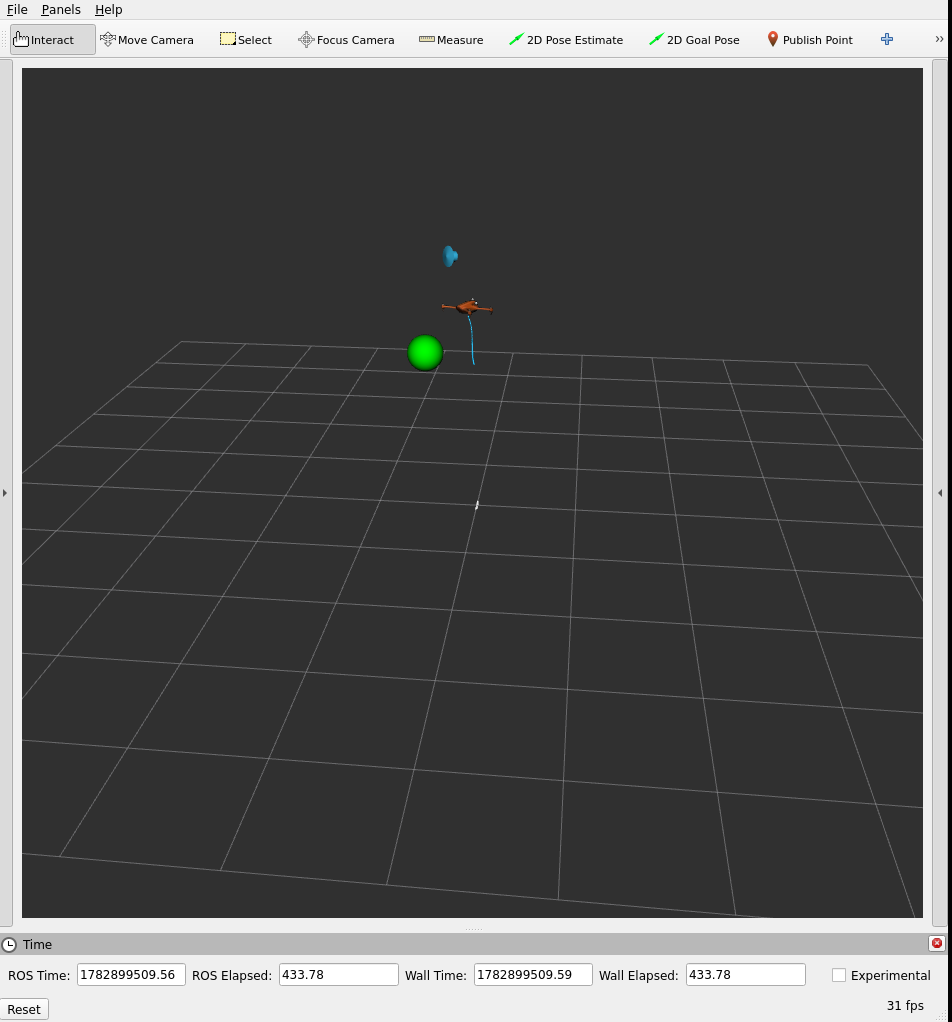
\includegraphics[width=0.82\textwidth]{images/rviz2_training_view.png}
\caption{Visualización en RViz2 del UAV simulado, la trayectoria reciente y el
marcador del objetivo durante una ejecución con Aerostack2.}
\label{fig:implementacion:rviz2_training_view}
\end{figure}

La Figura~\ref{fig:implementacion:rviz2_training_view} muestra un ejemplo de la
visualización empleada durante las pruebas. El marcador verde representa el
objetivo de navegación y el modelo del UAV permite comprobar de forma cualitativa
si el movimiento observado es coherente con las acciones enviadas por el entorno.

TensorBoard se emplea como herramienta de monitorización de las métricas emitidas
por Stable-Baselines3 y por los monitores vectorizados. En las ejecuciones en las
que PPO alcanza suficientes pasos para completar una primera actualización, esta
herramienta permite inspeccionar magnitudes como recompensa media por episodio,
longitud media de episodio y otros escalares registrados. Sin embargo, la
interpretación de TensorBoard debe realizarse junto con los ficheros de monitor y
los diagnósticos del entorno. Una curva ausente o congelada puede indicar que el
entrenamiento no ha alcanzado un \emph{rollout} completo, que el proceso se ha
bloqueado durante un reset o que el simulador ha dejado de producir transiciones
válidas.

\begin{table}[H]
\centering
\small
\setlength{\tabcolsep}{4pt}
\renewcommand{\arraystretch}{1.15}
\begin{tabular}{p{0.25\textwidth} p{0.62\textwidth}}
\hline
\textbf{Herramienta} & \textbf{Uso en el trabajo} \\
\hline
ROS 2 & Comunicación entre nodos, servicios, acciones y flujos de datos del sistema robótico. \\
Aerostack2 & Capa aérea reutilizada para armado, modos de vuelo, control y simulación. \\
AS2 Multirotor Simulator & Simulación dinámica del multirrotor usado como fuente de experiencia. \\
Gymnasium & Interfaz estándar del entorno de aprendizaje por refuerzo. \\
Stable-Baselines3 & Implementación de PPO y utilidades de entrenamiento. \\
TensorBoard & Monitorización de escalares y evolución de métricas durante ejecuciones PPO. \\
RViz2 & Visualización cualitativa del UAV, el objetivo y la trayectoria en el espacio simulado. \\
\hline
\end{tabular}
\caption{Herramientas principales utilizadas durante la implementación y validación.}
\label{tab:implementacion:herramientas}
\end{table}


\section{Implementación del entorno de aprendizaje} \label{sct:implementacion:entorno}

La clase \texttt{AS2TestEnv} materializa el diseño del
Capítulo~\ref{chp:diseno}. En lugar de volver a justificar los espacios de
observación y acción, esta sección se centra en cómo se ejecuta el contrato en el
código. El entorno registra \texttt{AS2TestEnv-v0}, define los espacios
\texttt{Box} correspondientes, aplica los límites configurados y encapsula las
operaciones de ciclo de vida que requiere Aerostack2.

Durante \texttt{reset}, el entorno prepara la interfaz robótica, arma el UAV,
activa el modo \emph{offboard}, ejecuta el despegue y devuelve la primera
observación normalizada. Cuando se habilita \texttt{randomize\_hover\_start}, la
posición inicial, la guiñada y el objetivo se muestrean dentro de los límites
configurados. Exp011 añade márgenes en XY y altura, junto con
\texttt{max\_start\_target\_distance}, para evitar episodios que comiencen junto
a fronteras problemáticas o con la observación saturada desde el primer paso.

Durante \texttt{step}, la acción recibida se recorta mediante \texttt{max\_vel} y
\texttt{max\_yaw\_vel}, se envía a Aerostack2 con \texttt{SpeedMotion} y se lee el
estado actualizado del UAV. Con esa información se calcula la recompensa, se
evalúan las condiciones de terminación y se generan campos de diagnóstico.

\begin{figure}[t]
\centering
\shorthandoff{<>}
\begin{tikzpicture}[
    node distance=1.05cm and 1.5cm,
    block/.style={
        rectangle,
        rounded corners,
        draw,
        align=center,
        minimum width=3.1cm,
        minimum height=0.8cm,
        font=\small
    },
    arrow/.style={-{Latex[length=2mm]}, thick}
]

\node[block] (reset) {\texttt{reset()}\\preparación del episodio};
\node[block, below=of reset] (obs0) {Observación inicial};
\node[block, below=of obs0] (policy) {Política PPO\\selección de acción};
\node[block, below=of policy] (action) {Acción limitada\\velocidad y yaw};
\node[block, below=of action] (step) {\texttt{step()}\\envío a AS2};
\node[block, below left=of step] (reward) {Recompensa\\distancia + terminales};
\node[block, below right=of step] (end) {Terminación o\\truncamiento};

\draw[arrow] (reset) -- (obs0);
\draw[arrow] (obs0) -- (policy);
\draw[arrow] (policy) -- (action);
\draw[arrow] (action) -- (step);
\draw[arrow] (step) -- (reward);
\draw[arrow] (step) -- (end);
\draw[arrow] (reward.west) .. controls +(-2.0,0) and +(-2.0,0) .. (policy.west);

\end{tikzpicture}
\shorthandon{<>}
\caption{Ciclo implementado de un episodio de aprendizaje por refuerzo sobre
\texttt{AS2TestEnv}.}
\label{fig:implementacion:ciclo_entorno}
\end{figure}

La Figura~\ref{fig:implementacion:ciclo_entorno} resume el flujo implementado.
La responsabilidad principal del entorno no es definir de nuevo el problema de
aprendizaje, sino convertir cada interacción de PPO en una operación robótica
acotada, observable y registrable.


\section{Diagnóstico del reinicio y de la accionabilidad} \label{sct:implementacion:diagnostico_reset}

La implementación añade un paso específico porque el entrenamiento solo
es válido si el UAV parte de un estado físico coherente y responde a las acciones
enviadas. Por este motivo, el entorno registra el método de reinicio, el camino
seguido, el estado del servicio, los errores residuales de posición y guiñada, el
desplazamiento físico, la longitud de trayectoria, la aceptación de comandos y la
altitud mínima. Estos campos permiten distinguir un fallo de aprendizaje de un
fallo previo de simulación o de accionabilidad.

El parámetro \texttt{reset\_max\_vel} separa la autoridad usada por los comandos
internos de reinicio de la velocidad máxima permitida a PPO. Por otra parte cabe
destacar que cuando la interfaz, acepta comandos pero el UAV no se desplaza de forma apreciable, 
el entorno falla
de forma cerrada y evita generar experiencia inválida.

El servicio \texttt{ResetSimulatorState}, añadido en el fork del simulador,
aplica una pose objetivo y reinicia velocidades, aceleraciones, fuerzas, pares,
motores, controlador, IMU y odometría. Sobre ese servicio se implementan
reintentos mediante \\ \texttt{reset\_service\_max\_attempts} y
\texttt{reset\_service\_retry\_backoff\_s}. Exp010 mostró que abortar tras un
fallo transitorio era demasiado frágil; Exp011 añadió reintentos, y Exp012 redujo
la frecuencia de reinicios forzados mediante un guard de acción en fronteras.

El guard de Exp012 modifica las acciones que empujan al UAV hacia fuera cuando se
aproxima a los límites XY o al techo de la escena. Las terminaciones por salida
de límites y baja altitud se mantienen como red de seguridad, pero dejan de ser
el mecanismo habitual para corregir a un agente aún no entrenado. A partir de
Exp013 el disparo de ambos guards es predictivo: se evalúa la posición estimada
como posición actual más velocidad medida por un horizonte configurable
(\texttt{bounds\_guard\_lookahead\_s},
\texttt{low\_altitude\_guard\_lookahead\_s}), y el empuje vertical dispone de
autoridad completa (\texttt{bounds\_guard\_vertical\_push\_speed}), porque los
datos de Exp012 mostraron que la inercia vertical atravesaba un guard puramente
reactivo (404 de 428 salidas de límites se produjeron por techo o suelo).

Para la ejecución vectorizada se implementa además el mecanismo de vigilancia de
comandos inactivos descrito en el diseño. Un hilo de fondo comprueba el tiempo
transcurrido desde la última referencia de movimiento enviada por cualquier vía
(pasos del agente, comandos de reinicio o sondas de accionabilidad); si el
vehículo está en vuelo y ese tiempo supera \texttt{idle\_command\_watchdog\_s},
publica referencias de velocidad nula a la cadencia de publicación configurada
hasta que el flujo normal se reanuda. La validación en vivo del mecanismo redujo
la deriva por referencias persistentes de 8,05 m a 0,27 m en una ventana de 20 s
sin comandos. El parámetro vale cero por defecto, de modo que la ejecución
monodron no crea el hilo ni altera su comportamiento.


\section{Infraestructura de entrenamiento y vectorización} \label{sct:implementacion:infraestructura_entrenamiento}

La infraestructura de entrenamiento se concentra en \texttt{ppo\_setup.py}. Este
módulo carga la configuración, crea los directorios de salida, instancia los
entornos, envuelve la ejecución con \texttt{VecMonitor} y construye el modelo PPO.
El registro de métricas se realiza sobre el entorno vectorizado para obtener
estadísticas de episodio agregadas sin duplicar lógica de monitorización en cada
instancia.

La vectorización se implementa mediante espacios de nombres ROS 2. A partir del
prefijo \texttt{drone} se generan instancias como \texttt{drone0},
\texttt{drone1}, \texttt{drone2}, ... , \texttt{droneN}, todas conectadas al mismo
simulador compartido. Esta solución evita lanzar un simulador por entorno y
mantiene la correspondencia entre instancia de Gymnasium y UAV simulado. La
implementación puede usar \texttt{DummyVecEnv} o \texttt{SubprocVecEnv} según la
configuración, aunque la validación inicial prioriza ejecuciones controladas
antes que paralelización agresiva.

El entrenamiento se ejecuta en dos pasos explícitos. Primero se lanza o verifica
el simulador con los scripts de AS2; después se ejecuta
\texttt{scripts/train\_ppo.py} con la configuración seleccionada. Para campañas
largas, \texttt{train\_ppo.py} acepta \texttt{--resume-from}, que reanuda desde
un \emph{checkpoint} explícito o desde el más reciente y calcula el número de
pasos restante hasta el total configurado (Stable-Baselines3 suma el argumento al
contador del \emph{checkpoint}, por lo que pasar el total completo duplicaría el
objetivo en cada reanudación).

El supervisor \texttt{scripts/supervise\_train.sh} automatiza tres mecanismos
sobre esa base. Ante un fallo del entrenamiento, reinicia el stack AS2 completo,
espera a que el servicio de reinicio de cada dron esté disponible y reanuda desde
el último \emph{checkpoint}. Mediante la variable \texttt{RECYCLE\_SECONDS}
aplica además un reciclado preventivo donde interrumpe el entrenamiento a intervalos
fijos y lo reanuda sobre un stack recién iniciado, de modo que cada tramo se
ejecuta sobre un simulador sin degradación acumulada; los reciclados se detectan
por el tiempo transcurrido, no solo por el código de salida, y no consumen el
presupuesto de reintentos por fallo. Por último, \texttt{DRONE\_NAMESPACES}
extiende el reinicio y la comprobación de salud a varios drones para las campañas
vectorizadas, e \texttt{INITIAL\_RESUME} permite sembrar una etapa del curriculum
con el modelo final de la etapa anterior cuando aún no existen \emph{checkpoints}
propios.

La validación inicial confirma que el pipeline puede crear el modelo PPO,
conectarse con AS2, enviar comandos de velocidad y generar trazas
monitorizables. Esta evidencia prueba la infraestructura de entrenamiento, no el
rendimiento final de la política; esa interpretación corresponde a los capítulos
de pruebas y resultados.

% !TEX root = ../tfg_etsiinf_NombreApellidos.tex
\chapter{Aplicación y validación de la arquitectura} \label{chp:pruebas}

Este capítulo aplica la infraestructura desarrollada a una tarea concreta de
control de velocidad para un UAV simulado. Mientras que el
Capítulo~\ref{chp:implementacion} verifica que los componentes están correctamente
implementados y pueden producir transiciones físicas válidas, aquí se analiza si
la arquitectura permite entrenar una política PPO para alcanzar un objetivo
relativo mediante comandos continuos de velocidad y guiñada. Esta aplicación
convierte la arquitectura en una infraestructura de experimentación: las observaciones, las
acciones, la recompensa, el reinicio y la monitorización se ejercitan de forma
conjunta bajo una misma tarea de control.

La validación distingue la disponibilidad de la infraestructura del
comportamiento de la política. Un entrenamiento solo es interpretable si cada
episodio comienza en un estado verificable y las acciones modifican físicamente
el estado del vehículo; sobre esa condición se pueden evaluar la aproximación al
objetivo, las terminaciones y las métricas de aprendizaje. Las secciones
siguientes presentan la formulación de la tarea, las salvaguardas y la
configuración empleada, así como los criterios con los que se analizan las
ejecuciones.

\section{Propósito y alcance de la aplicación} \label{sct:aplicacion:alcance}

La aplicación de validación consiste en entrenar una política PPO que recibe el
estado relativo del UAV respecto de un objetivo y emite velocidades lineales y
de guiñada. El entrenamiento se ejecuta sobre \texttt{AS2TestEnv}, que traduce
cada acción de la política en una referencia para Aerostack2 y devuelve la
observación, la recompensa y el estado de terminación correspondientes. De este
modo, la tarea exige simultáneamente que el canal de control sea accionable, que
el ciclo de reinicio sea fiable y que la formulación de aprendizaje proporcione
una señal útil para la navegación local.

Esta aplicación no se plantea como una demostración aislada de que el proceso de
entrenamiento se inicia, sino como una validación integrada del objetivo del
trabajo. Una ejecución adecuada debe generar episodios trazables, conservar las
condiciones de seguridad y permitir evaluar si la política reduce la distancia
al objetivo y alcanza la región de éxito. Los apartados posteriores concretan
esta tarea mediante la formulación de control, la recompensa, el curriculum, las
protecciones de frontera, la configuración de PPO y las métricas de aceptación.

\section{Formulación de la tarea de control} \label{sct:aplicacion:formulacion}

El problema de control se formula como una tarea de navegación local hacia un
objetivo relativo. En este contexto, navegación local significa que el agente no
recibe una misión global completa ni una trayectoria predefinida con todos sus
puntos intermedios, sino la relación geométrica entre el estado actual del UAV y
un objetivo inmediato. A partir de esa relación, el agente debe emitir comandos
de velocidad que acerquen el vehículo al objetivo y mantengan una orientación
coherente con la dirección de desplazamiento.

Antes de definir formalmente las observaciones y acciones, conviene distinguir
las magnitudes básicas que describen el movimiento de un multirrotor. La posición
indica dónde se encuentra el UAV en el espacio; la velocidad indica cómo cambia
esa posición; y la orientación describe la rotación del vehículo respecto a sus
ejes. En un dron se suelen emplear tres ángulos principales, denominados
\emph{roll}, \emph{pitch} y \emph{yaw}. El \emph{roll} representa la inclinación lateral,
el \emph{pitch} la inclinación hacia delante o hacia atrás, y el \emph{yaw} la
rotación alrededor del eje vertical. La Figura~\ref{fig:diseno:pose_drone}
resume esta idea de pose del dron mediante una representación conceptual tomada
de ResearchGate.\footnote{Imagen disponible en ResearchGate:
\url{https://www.researchgate.net/figure/A-conceptual-representation-of-drone-pose-A-drone-here-represented-by-a-DJI-Mavic-2-is_fig1_356985671}. Según la página consultada, la figura aparece con licencia Creative Commons Attribution-NonCommercial-ShareAlike 4.0 International.}

\begin{figure}[t]
    \centering
    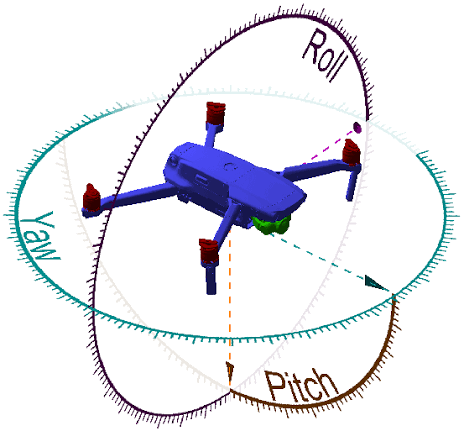
\includegraphics[width=0.58\textwidth]{images/drone_pose_roll_pitch_yaw.png}
    \caption{Representación conceptual de la pose de un dron mediante los ángulos
    de \emph{roll}, \emph{pitch} y \emph{yaw}. Fuente: ResearchGate.}
    \label{fig:diseno:pose_drone}
\end{figure}

En el presente trabajo no se controla directamente la actitud completa del dron
ni las velocidades de giro de cada rotor. La acción se define a un nivel de abstracción superior, en el que el agente
genera velocidades lineales y una velocidad de guiñada. Esta elección sitúa el
aprendizaje por refuerzo por encima del control de bajo nivel y delega en
Aerostack2 la ejecución de los comandos sobre el simulador. Desde el punto de
vista del diseño, esta separación reduce la
complejidad del problema aprendido y mantiene la compatibilidad con la interfaz
de control de velocidad disponible.

La formulación distingue también entre la dirección frontal del UAV y la
dirección real de avance. Un dron puede desplazarse hacia un objetivo aunque su
eje frontal no esté alineado con la trayectoria seguida. El criterio de
\emph{path-facing}, ilustra la
diferencia entre ambas magnitudes y la relación con el error de guiñada. En la
formulación final de la solución no se exige el seguimiento de una trayectoria: la guiñada se
considera únicamente al evaluar el éxito terminal. La
Figura~\ref{fig:aplicacion:target_path_facing} representa esta relación
geométrica.


\begin{figure}[t]
\centering
\shorthandoff{<>}
\begin{tikzpicture}[
    x=1cm,
    y=1cm,
    axis/.style={-{Latex[length=2mm]}, thick, gray},
    rel/.style={-{Latex[length=2.5mm]}, very thick, blue},
    front/.style={-{Latex[length=2.5mm]}, very thick, green!55!black},
    path/.style={-{Latex[length=2.5mm]}, very thick, orange!85!black},
    helper/.style={dashed, gray!65},
    label/.style={font=\small},
    smalllabel/.style={font=\scriptsize}
]

\coordinate (uav) at (0,0);
\coordinate (target) at (6.2,2.5);
\coordinate (front) at (2.0,0.35);
\coordinate (pathvec) at (2.0,0.85);

% Axes
\draw[axis] (-0.6,0) -- (7.0,0) node[right, label] {$x$};
\draw[axis] (0,-0.5) -- (0,3.2) node[above, label] {$y$};

% UAV and target
\begin{scope}[shift={(uav)}, rotate=10]
    \draw[fill=gray!20, thick] (0.48,0) -- (-0.32,0.22) -- (-0.32,-0.22) -- cycle;
\end{scope}
\node[label, below left=0.12cm of uav] {UAV};
\filldraw[red] (target) circle (2.3pt);
\node[label, red, above right=0.05cm of target] {objetivo};

% Projection helpers
\draw[helper] (target) -- (6.2,0);
\draw[helper] (target) -- (0,2.5);

% Main vectors
\draw[rel] (uav) -- (target);
\draw[front] (uav) -- (front);
\draw[path] (uav) -- (pathvec);

% Angle arcs
\draw[->, thick, green!55!black] (0.85,0) arc[start angle=0,end angle=10,radius=0.85];
\draw[->, thick, orange!85!black] (1.2,0) arc[start angle=0,end angle=23,radius=1.2];
\draw[<->, thick, red!70!black] (1.55,0.27) arc[start angle=10,end angle=23,radius=1.58];

% Compact legend below the plot, outside the geometry
\begin{scope}[shift={(0,-1.25)}]
    \draw[rel] (0.0,0.0) -- (0.65,0.0);
    \node[label, anchor=west] at (0.85,0.0) {vector relativo $(d_x,d_y)$};

    \draw[front] (5.2,0.0) -- (5.85,0.0);
    \node[label, anchor=west] at (6.05,0.0) {dirección frontal};

    \draw[path] (0.0,-0.55) -- (0.65,-0.55);
    \node[label, anchor=west] at (0.85,-0.55) {dirección de avance};

    \draw[<->, thick, red!70!black] (5.2,-0.55) -- (5.85,-0.55);
    \node[label, anchor=west] at (6.05,-0.55) {error $e_{\mathrm{yaw}}$};
\end{scope}

\end{tikzpicture}
\shorthandon{<>}
\caption{Relación geométrica entre el UAV, el objetivo relativo, la dirección de
avance y la orientación de guiñada utilizada en el criterio de
\emph{path-facing}.}
\label{fig:aplicacion:target_path_facing}
\end{figure}

La acción se define mediante el vector continuo
\[
    a = [v_x, v_y, v_z, v_{\mathrm{yaw}}].
\]
Las tres primeras componentes representan velocidades lineales en los ejes
cartesianos y la cuarta representa la velocidad angular de guiñada. El espacio de
acciones se acota mediante los parámetros \texttt{max\_vel} y
\texttt{max\_yaw\_vel}, lo que introduce una restricción explícita de diseño
sobre la magnitud de las órdenes que el agente puede emitir. Esta acotación es
necesaria porque una política de aprendizaje por refuerzo puede proponer acciones
arbitrarias dentro de su espacio de salida, mientras que el sistema físico o
simulado solo debe recibir comandos dentro de un rango admisible.

La observación se define mediante el vector relativo
\[
    o = [d_x, d_y, d_z, d_{\mathrm{yaw}}].
\]
Cada componente se normaliza en el intervalo $[-1, 1]$. Las tres primeras
componentes codifican el desplazamiento relativo hacia el objetivo, y la cuarta
codifica la diferencia relativa de guiñada. La normalización reduce la dependencia
respecto a la escala concreta del escenario y proporciona al agente entradas con
rangos homogéneos, una condición práctica para estabilizar el tratamiento de las
observaciones por parte del algoritmo de aprendizaje.

\section{Recompensa y condiciones de finalización} \label{sct:aplicacion:recompensa}

La recompensa final usada en la fase de experimentación principal se diseña para
mantener una señal mínima e interpretable. En
cada paso se penaliza únicamente la distancia normalizada al objetivo. Para ello, si
$d_t$ representa la distancia euclídea entre el UAV y el objetivo, y
$d_{\max}$ representa la distancia máxima de normalización. A partir de ambas
magnitudes se obtiene
\begin{equation}
    d_{\mathrm{norm}} = \min\left(\frac{d_t}{d_{\max}}, 1\right),
    \qquad
    r_{\mathrm{dist}} = -d_{\mathrm{norm}}.
\end{equation}
En la interfaz Gymnasium implementada, $d_{\max}$ se calcula a partir del límite espacial de
posición del escenario, de forma que la distancia normalizada queda acotada en el
intervalo $[0,1]$.

La interfaz Gymnasium conserva la capacidad de calcular términos adicionales, como progreso,
seguridad vertical o coherencia de guiñada con la dirección de movimiento. Sin
embargo, esos términos se desactivan a partir de Exp010 y en toda la campaña
principal para evitar que el agente optimice una recompensa de shaping distinta
de la tarea principal. La guiñada se mantiene como requisito terminal suave. Cuando el UAV alcanza la
región objetivo, la bonificación de éxito se reduce en función del error de
guiñada. Si
$e_{\mathrm{yaw}}$ representa el error angular normalizado, la recompensa terminal
de éxito se calcula mediante
\begin{equation}
    r_{\mathrm{success}} =
    R_{\mathrm{success}} -
    w_{\mathrm{yaw}} \frac{|e_{\mathrm{yaw}}|}{\pi}.
\end{equation}

La expresión final aplicada desde Exp010 en adelante incorpora las
condiciones terminales del episodio de la forma siguiente.
\begin{equation}
    r_t =
    \begin{cases}
        -P_{\mathrm{oob}}, & \text{si el UAV sale de los límites del escenario},\\
        -P_{\mathrm{oob}}, & \text{si el UAV entra en baja altitud insegura},\\
        r_{\mathrm{success}}, &
            \text{si } d_t < d_{\mathrm{threshold}},\\
        -d_{\mathrm{norm}}, & \text{en el resto de pasos}.
    \end{cases}
\end{equation}
El truncamiento por alcanzar \texttt{max\_steps} no introduce una recompensa
adicional, sino que limita la duración del episodio cuando no se ha alcanzado una
condición terminal. El Cuadro~\ref{tab:aplicacion:componentes_recompensa} resume los
componentes de esta formulación y su efecto esperado.

\begin{table}[t]
\centering
\small
\setlength{\tabcolsep}{4pt}
\renewcommand{\arraystretch}{1.15}
\begin{tabular}{p{0.24\textwidth} p{0.25\textwidth} p{0.19\textwidth} p{0.22\textwidth}}
\hline
\textbf{Componente} & \textbf{Expresión} & \textbf{Condición} & \textbf{Efecto esperado} \\
\hline

Penalización por distancia &
$r_{\mathrm{dist}} = -d_{\mathrm{norm}}$ &
En cada paso &
Favorece que el UAV reduzca progresivamente la distancia al objetivo. \\

Bonificación por éxito &
$R_{\mathrm{success}} - w_{\mathrm{yaw}} |e_{\mathrm{yaw}}|/\pi$ &
Si $d_t < d_{\mathrm{threshold}}$ &
Premia alcanzar la región objetivo y reduce la bonificación si la guiñada terminal es inadecuada. \\

Penalización por salida de límites &
$-P_{\mathrm{oob}}$ &
Si el UAV supera los límites del escenario &
Desincentiva trayectorias inseguras o alejadas de la zona de entrenamiento. \\

Penalización por baja altitud insegura &
$-P_{\mathrm{oob}}$ &
Si el UAV desciende por debajo del umbral inseguro &
Evita que el aprendizaje explote estados cercanos al suelo o físicamente no válidos. \\

Truncado temporal &
Sin recompensa adicional &
Si se alcanza el número máximo de pasos &
Limita la duración del episodio cuando no se alcanza una condición terminal. \\

\hline
\end{tabular}
\caption{Componentes de la función de recompensa y condiciones de finalización de la interfaz Gymnasium.}
\label{tab:aplicacion:componentes_recompensa}
\end{table}

\section{Curriculum de distancia} \label{sct:aplicacion:curriculum}

Con la recompensa mínima $-d_{\mathrm{norm}}$, la única señal positiva del
problema es la bonificación terminal, y su densidad depende de la probabilidad de
que la exploración alcance la esfera de éxito de 0,4 m. Con separaciones
inicio--objetivo de hasta 5 m esa probabilidad es demasiado baja para arrancar el
gradiente con la tasa de aprendizaje configurada. El diseño adopta por ello un
curriculum de distancia \cite{bengio2009curriculum} en tres etapas: la primera acota la separación máxima a
2,5 m, de modo que un vuelo directo requiere del orden de 25 pasos; las dos
siguientes amplían el límite a 3,5 m y finalmente a 5,0 m. Cada
etapa se inicializa con el modelo final de la anterior (\emph{warm start}) y
todas mantienen la separación mínima de 1,0 m, de forma que la distribución de
episodios de una etapa contiene a la anterior y la política no olvida los
objetivos cercanos al aprender los lejanos.

\section{Protecciones de frontera} \label{sct:aplicacion:guards}

La observación relativa tiene una consecuencia de diseño que los primeros
experimentos hicieron explícita y es que el agente no puede percibir los límites del
escenario. Una terminación por salida de límites es, desde el punto de vista de
la política, un castigo imprevisible aplicado en estados que no se distinguen de
los estados seguros, por lo que la función de valor no puede anticiparla. Además,
cada una de estas terminaciones obliga a un reinicio mediante el servicio del
simulador, con un coste de decenas de segundos y efectos acumulativos sobre la
plataforma. Por ambos motivos, el diseño sustituye la muerte en frontera por una
protección activa: un \emph{guard} de acción que, cerca de los límites, reemplaza
la componente de velocidad saliente por un empuje hacia el interior.

El guard se diseña con disparo predictivo. La versión reactiva, que actúa cuando
la posición cruza una línea de guardia, resultó insuficiente en el eje vertical ya que
la plataforma invierte la velocidad con lentitud y la inercia atraviesa el margen
antes de que la orden correctora surta efecto. Por ello el disparo evalúa la
posición \emph{predicha}, calculada como posición actual más velocidad medida por
un horizonte de anticipación, y el empuje vertical utiliza la autoridad completa
de velocidad disponible. Las terminaciones por salida de límites y por baja
altitud se conservan intactas como red de seguridad final, pero con el guard
activo pasan de ser el desenlace dominante (80--93\,\% de los episodios en
Exp010--Exp011) a ser residuales, lo que elimina a la vez el ruido inaprendible
de la recompensa y la mayor parte de los reinicios costosos.

\section{Extensión a ejecución vectorizada} \label{sct:aplicacion:vectorizacion}

La ejecución vectorizada se diseña para permitir varias instancias lógicas del
entorno sobre un único simulador compartido. El diseño utiliza espacios de nombres
diferenciados, \texttt{drone0} a \texttt{droneN}, de forma que cada UAV simulado
pueda ser identificado y gobernado de manera independiente dentro de la misma
infraestructura ROS 2. Esta organización reduce la necesidad de duplicar toda la
infraestructura del simulador, pero exige tratar con cuidado la inicialización de
ROS 2, los nombres de los drones y la sincronización entre episodios.

La Figura~\ref{fig:aplicacion:vectorizacion} resume esta organización. Cada
instancia lógica mantiene su propio espacio de nombres, pero todas comparten la
infraestructura física de simulación, por lo que sus reinicios y sus tiempos de
paso deben coordinarse.

\begin{figure}[t]
\centering
\shorthandoff{<>}
\begin{tikzpicture}[
    node distance=1.1cm and 1.4cm,
    block/.style={
        rectangle,
        rounded corners,
        draw,
        align=center,
        minimum width=2.8cm,
        minimum height=0.8cm,
        font=\small
    },
    smallblock/.style={
        rectangle,
        rounded corners,
        draw,
        align=center,
        minimum width=2.4cm,
        minimum height=0.7cm,
        font=\small
    },
    arrow/.style={-{Latex[length=2mm]}, thick}
]

\node[block] (vec) {Entorno vectorizado\\\texttt{SyncVectorEnv}/\texttt{DummyVecEnv}};

\node[smallblock, below left=of vec] (env0) {Instancia 0\\\texttt{drone0}};
\node[smallblock, below=of vec] (env1) {Instancia 1\\\texttt{drone1}};
\node[smallblock, below right=of vec] (env2) {Instancia 2\\\texttt{drone2}};

\node[block, below=2.0cm of env1] (ros) {ROS 2\\espacios de nombres};
\node[block, below=of ros] (sim) {AS2 Multirotor\\Simulator compartido};

\draw[arrow] (vec) -- (env0);
\draw[arrow] (vec) -- (env1);
\draw[arrow] (vec) -- (env2);

\draw[arrow] (env0) -- (ros);
\draw[arrow] (env1) -- (ros);
\draw[arrow] (env2) -- (ros);

\draw[arrow] (ros) -- (sim);

\node[draw, dashed, rounded corners, fit=(env0)(env1)(env2), inner sep=0.25cm,
      label={[font=\small]right:Instancias lógicas del entorno}] {};

\end{tikzpicture}
\shorthandon{<>}
\caption{Extensión vectorizada mediante instancias lógicas asociadas a espacios
de nombres diferenciados sobre una infraestructura de simulación compartida.}
\label{fig:aplicacion:vectorizacion}
\end{figure}

La elección del mecanismo de vectorización viene determinada por una propiedad
del simulador: opera en tiempo de reloj real, de modo que cada paso del entorno
consume la duración física configurada (0,2 s) con independencia del proceso que
lo invoque. Esta propiedad invalida en este sistema el razonamiento habitual a
favor de la vectorización secuencial (\texttt{SyncVectorEnv} en Gymnasium,
\texttt{DummyVecEnv} en Stable-Baselines3), cuyo beneficio procede de agrupar las
observaciones para una única inferencia por lotes: con un simulador de reloj
real, $N$ entornos secuenciales tardan $N$ veces el paso físico en producir $N$
muestras, es decir, el mismo caudal de muestreo que un solo entorno. Por ello el
diseño adopta \texttt{SubprocVecEnv}, que ejecuta los pasos de los $N$ entornos
en paralelo real manteniendo la inferencia por lotes, con la expectativa
(verificada experimentalmente) de multiplicar el muestreo por el número de
drones.

El paso vectorizado en paralelo introduce, sin embargo, un modo de fallo propio
de los simuladores de reloj real, el avance en \emph{lockstep}. Cuando uno de los
entornos ejecuta su reinicio, es una operación que tarda decenas de
segundos, el paso vectorizado queda bloqueado para todos; durante ese intervalo
los demás drones no reciben órdenes nuevas mientras el mundo sigue avanzando, y
el controlador de Aerostack2 mantiene la última referencia de velocidad como
consigna activa. El diseño incorpora por ello un mecanismo de vigilancia
(\emph{watchdog}) de comandos inactivos, es decir,si un entorno en vuelo supera un umbral
de tiempo sin emitir referencias de movimiento, el mecanismo publica una consigna
de velocidad nula de forma periódica hasta que el flujo normal de comandos se
reanuda. El umbral se dimensiona por encima de la duración del paso, de modo que
el mecanismo permanece inerte durante la operación normal y solo actúa en los
huecos de \emph{lockstep}; en ejecución monodron queda desactivado y el
comportamiento del entorno es idéntico al de la fase anterior.

\section{Configuración del entrenamiento PPO} \label{sct:aplicacion:ppo}

La configuración de PPO se materializa en
\texttt{configs/train\_ppo.yaml}. El Capítulo~\ref{chp:state-of-the-art}
justifica la elección del algoritmo; esta sección se limita a documentar cómo se
parametriza su uso dentro de la arquitectura implementada y cómo se preserva la
trazabilidad de cada ejecución.

La configuración se divide en tres bloques principales. El bloque
\texttt{experiment} define el nombre del experimento, la semilla y el directorio
raíz de salida. El bloque \texttt{environment} agrupa los parámetros del entorno,
incluyendo el identificador \texttt{AS2TestEnv-v0}, el número de instancias
vectorizadas, el prefijo de espacio de nombres, los límites de posición y
velocidad, la duración de cada paso, el objetivo, las condiciones de éxito y las
penalizaciones de seguridad. El bloque \texttt{ppo} contiene los hiperparámetros
del algoritmo, como la tasa de aprendizaje, el número de pasos por actualización,
el tamaño de lote, el factor de descuento, el rango de \emph{clipping} y la
arquitectura de las redes de política y valor.

\begin{table}[H]
\centering
\small
\setlength{\tabcolsep}{4pt}
\renewcommand{\arraystretch}{1.15}
\begin{tabular}{p{0.28\textwidth} p{0.22\textwidth} p{0.40\textwidth}}
\hline
\textbf{Parámetro} & \textbf{Valor base} & \textbf{Función} \\
\hline
\texttt{total\_timesteps} & \texttt{1000000} & Duración máxima de la campaña de entrenamiento. \\
\texttt{learning\_rate} & \texttt{3.0e-05} & Tamaño de actualización de los parámetros de PPO. \\
\texttt{n\_steps} & \texttt{512} & Número de pasos recogidos antes de cada actualización. \\
\texttt{batch\_size} & \texttt{32} & Tamaño de lote usado durante la optimización. \\
\texttt{clip\_range} & \texttt{0.2} & Límite de variación entre política antigua y política nueva. \\
\texttt{use\_sde} & \texttt{true} & Activación de exploración dependiente del estado. \\
\texttt{net\_arch} & \texttt{[128, 128]} & Capas ocultas de las redes de política y valor. \\
\hline
\end{tabular}
\caption{Principales parámetros PPO definidos en la configuración base de entrenamiento.}
\label{tab:aplicacion:parametros_ppo}
\end{table}

El Cuadro~\ref{tab:aplicacion:parametros_ppo} recoge los parámetros más
representativos de la configuración base. Estos valores no deben interpretarse
como una optimización definitiva del algoritmo, sino como una configuración
inicial trazable y reproducible para validar la infraestructura de entrenamiento.
Los capítulos de pruebas y resultados son los que deben determinar si una
configuración concreta produce aprendizaje útil, estabilidad suficiente o
necesidad de ajuste.

A partir de Exp010 se utiliza una configuración ajustada con tasa de aprendizaje \texttt{3.0e-05},
\texttt{n\_steps=512}, \texttt{batch\_size=32}, \texttt{n\_epochs=5},
\texttt{ent\_coef=0.0}, exploración SDE y redes MLP de dos capas de 128 unidades
por rama. Las configuraciones Exp010, Exp011 y Exp012 mantienen estos
hiperparámetros y modifican principalmente propiedades del entorno y de la tarea,
como la recompensa mínima, la randomización completa, los márgenes de muestreo,
el límite de distancia inicio--objetivo, los guards de acción y la reanudación de
entrenamiento. Esta separación evita mezclar ajustes del algoritmo con cambios en
las condiciones de interacción del UAV.

La configuración también explicita decisiones de que afectan a la
reproducibilidad. El entrenamiento se fija inicialmente en CPU, coherente con el
uso de políticas MLP y con la recomendación habitual de Stable-Baselines3 para
evitar sobrecostes de GPU en redes no convolucionales. Además, se separan los
directorios de \emph{logs}, monitorización y \emph{checkpoints}, lo que permite
analizar una ejecución sin depender únicamente de la salida estándar del proceso.
Esta estructura facilita repetir experimentos, comparar configuraciones y aislar
fallos entre simulación, interfaz Gymnasium y algoritmo.


\section{Métricas y criterios de interpretación} \label{sct:aplicacion:metricas}

Las métricas empleadas combinan indicadores de aprendizaje e indicadores de
infraestructura. En el primer grupo se encuentran la recompensa por episodio, la
longitud de episodio, la tasa de éxito y la distancia final al objetivo. En el
segundo grupo se registran razones de terminación, desplazamiento físico,
longitud de trayectoria, altitud mínima, ratio de comandos aceptados, método de
reset y clase de fallo. Esta separación permite determinar si una ejecución
fracasa porque la política todavía no resuelve la tarea o porque la arquitectura no
está entregando transiciones físicamente válidas.

Las curvas de TensorBoard se utilizan como evidencia complementaria, no como
única prueba de aprendizaje. En particular, las métricas
\texttt{rollout/ep\_rew\_mean} y \texttt{rollout/ep\_len\_mean} permiten
observar tendencias agregadas, mientras que los campos de monitor por episodio
permiten explicar esas tendencias mediante razones de terminación, distancia
final, éxitos, salidas de límites o eventos de baja altitud. Esta combinación es
necesaria porque una curva plana de recompensa puede deberse a una política que
no aprende, pero también a episodios dominados por terminaciones de seguridad o
por reinicios costosos del simulador.

El criterio de aceptación para un entrenamiento no se reduce a que el proceso de
Python siga ejecutándose. Una ejecución solo se considera apta para análisis de
aprendizaje si la arquitectura establece episodios desde estados válidos, si las acciones
producen movimiento físico medible, si los fallos de reset no se ocultan como
episodios válidos y si las métricas de monitorización permiten reconstruir lo
ocurrido. En caso contrario, el resultado se documenta como evidencia de
integración y se utiliza para mejorar la arquitectura antes de extraer conclusiones
sobre PPO.

% !TEX root = ../tfg_etsiinf_NombreApellidos.tex
\chapter{Resultados} \label{chp:resultados}

Este capítulo presenta los resultados obtenidos mediante la estrategia de pruebas
definida previamente. La exposición distingue entre resultados de infraestructura
y resultados de aprendizaje. Esta distinción es esencial en el presente trabajo:
la capacidad de lanzar PPO y generar métricas no implica por sí misma que se haya
obtenido una política robusta, especialmente cuando los experimentos revelan
problemas de reinicio, accionabilidad o coherencia física del simulador.

\section{Validación funcional de la infraestructura} \label{sct:resultados:validacion}

Las primeras pruebas confirman que la infraestructura básica es operativa. El
entorno puede instanciarse como entorno Gymnasium, conectarse con Aerostack2,
armar el UAV, activar el modo \emph{offboard}, ejecutar despegue, enviar comandos
de velocidad y registrar métricas mediante los mecanismos de monitorización. Esta
validación funcional demuestra que la integración entre Gymnasium,
Stable-Baselines3, ROS 2 y Aerostack2 es viable.

No obstante, los resultados también muestran que la validez de un entrenamiento
depende de condiciones adicionales. En las primeras ejecuciones se observaron
éxitos triviales cuando el objetivo estaba demasiado cerca de la pose de
despegue, ausencia de escalares de TensorBoard cuando PPO no alcanzaba suficientes
pasos de \emph{rollout}, y bucles de episodios fuera de límites cuando el reset no
garantizaba un estado inicial seguro. Las iteraciones posteriores permitieron
certificar el reinicio mediante el servicio del simulador y ejecutar
entrenamientos más largos, pero también revelaron que las salidas de límites y la
degradación acumulada por reinicios de servicio podían dominar el comportamiento
observado. Estos resultados condujeron a separar el problema en dos niveles:
primero validar el ciclo físico de episodio y después analizar el aprendizaje.

\section{Matriz de experimentos PPO} \label{sct:resultados:matriz_experimentos}

El Cuadro~\ref{tab:resultados:experimentos} resume la evolución de los
experimentos principales. La tabla no debe interpretarse como una búsqueda lineal
de hiperparámetros, sino como una secuencia de validación en la que cada ejecución
revela una propiedad de la infraestructura.

\begin{table}[H]
\centering
\scriptsize
\setlength{\tabcolsep}{2.5pt}
\renewcommand{\arraystretch}{1.12}
\begin{tabular}{p{0.10\textwidth} p{0.21\textwidth} p{0.25\textwidth} p{0.34\textwidth}}
\hline
\textbf{Experimento} & \textbf{Objetivo} & \textbf{Resultado observado} & \textbf{Interpretación técnica} \\
\hline
Exp001 & Smoke PPO con configuración inicial. & Episodios de éxito en un paso y métricas insuficientes. & El objetivo estaba demasiado cerca del estado inicial; no era una tarea de navegación útil. \\
Exp002 & Objetivo desplazado y TensorBoard en prueba corta. & Primeros episodios útiles, después bucles de salida de límites. & El pipeline generaba artefactos, pero el reset no garantizaba inicio seguro tras OOB. \\
Exp003 & Introducir \texttt{fixed\_start\_pose}. & Entrenamiento corto completado con monitor, TensorBoard y \emph{checkpoints}. & El reset determinista resolvió el bucle inmediato de OOB en una prueba acotada. \\
Exp004 & Target más lejano y marcador RViz. & Se mejoró la observabilidad del objetivo y de métricas. & RViz y marcadores ayudan a validar cualitativamente la escena, no sustituyen métricas. \\
Exp005 & Target estable a 2 m y reset en vuelo. & Primeras evidencias de éxito real hacia un punto, con incidencias de reset. & El reset en vuelo evitó bloqueos de aterrizaje, pero la robustez seguía siendo limitada. \\
Exp006 & Mejorar estabilidad y evitar fallback problemático. & Se detectó bloqueo asociado a \texttt{go\_to}. & El retorno a pose inicial debía evitar comportamientos bloqueantes. \\
Exp007 & Gate largo tras eliminar \texttt{go\_to}. & Fallo acotado por timeout de reset por velocidad. & El entrenamiento ya no quedaba bloqueado, pero el reset seguía sin ser fiable para runs largos. \\
Exp008 & Reset más robusto con target de 2 m. & Persisten timeouts de reset. & La dificultad seguía siendo alta para depurar aprendizaje si el reset fallaba. \\
Exp008a & Curriculum de 0,5 m y diagnóstico ampliado. & Mejora parcial, pero aparecen bloqueos de reset y accionabilidad. & El cuello de botella pasa de PPO a la interacción reset--controlador--simulador. \\
Exp009 & Primer gate PPO sobre el stack de reset certificado. & Ejecución de 5102 pasos de monitor, 126 episodios y finalización correcta del proceso. & Se valida la infraestructura de episodio; la tasa de éxito observada, 21/126 episodios, no se interpreta todavía como política robusta. \\
Exp010 & Recompensa mínima alineada con el tutor, randomización completa e hiperparámetros revisados. & Se registran 12852 pasos y 427 episodios antes del fallo; 359 terminan fuera de límites y 65 por baja altitud. & El diseño de recompensa queda alineado, pero las fronteras no observables y el coste de teleport dominan la experiencia. \\
Exp011 & Muestreo en área segura y límite de distancia inicio--objetivo para evitar saturación de observaciones. & Se registran 21347 pasos y 637 episodios; 512 terminan fuera de límites, 121 por baja altitud y solo 3 en éxito. & La saturación inicial se corrige parcialmente, pero el problema estructural de terminaciones y reinicios repetidos persiste. \\
Exp012 & Guard de acción en límites, corredor vertical ampliado, reanudación desde \emph{checkpoint} y supervisor. & Experimento en ejecución durante la redacción de esta versión. & La hipótesis evaluada es reducir reinicios de servicio y aislar mejor el aprendizaje de PPO de los fallos de infraestructura. \\
\hline
\end{tabular}
\caption{Resumen de experimentos principales y su interpretación.}
\label{tab:resultados:experimentos}
\end{table}

\section{Resultados de entrenamiento y monitorización} \label{sct:resultados:entrenamiento}

Los experimentos muestran que la infraestructura de entrenamiento produce
artefactos analizables cuando alcanza suficiente número de pasos: ficheros de
monitor, eventos de TensorBoard, \emph{checkpoints} y modelos finales en
pruebas acotadas. En particular, las ejecuciones iniciales permiten comprobar que
TensorBoard y los monitores de episodio funcionan cuando PPO completa
\emph{rollouts} suficientes, mientras que Exp009 confirma que el stack de reset
certificado puede sostener una ejecución PPO completa de 5000 pasos. Sin embargo,
la presencia de estos artefactos no implica aprendizaje estable: debe analizarse
junto con las razones de terminación, la longitud de episodio, la distancia
final, la tasa de éxito y los diagnósticos de reset.

Las métricas agregadas de TensorBoard son especialmente útiles para interpretar
Exp010 y Exp011, porque permiten observar si la recompensa media, la longitud de
episodio o la tasa de éxito muestran una tendencia temporal. En las condiciones
registradas, la evidencia disponible no debe presentarse como una política final
aprendida, sino como una secuencia de diagnóstico: Exp010 muestra que la
formulación de recompensa e hiperparámetros ya está alineada con el criterio del
tutor, pero que la experiencia queda dominada por salidas de límites; Exp011
reduce la saturación de observaciones mediante un área de muestreo más segura,
pero no elimina el predominio de terminaciones no deseadas. Por ello, las curvas
de TensorBoard deben leerse junto con los ficheros de monitor y con la matriz de
experimentos, no de forma aislada.

La comparación cuantitativa entre Exp010 y Exp011 muestra una mejora parcial,
pero insuficiente. En Exp010 se registran 427 episodios, con 359 terminaciones
por salida de límites, 65 por baja altitud insegura y 3 éxitos. La recompensa
media por episodio es aproximadamente \(-31{,}36\), la longitud media es de
30,10 pasos y la distancia final media al objetivo es de 5,41 m. En Exp011 se
registran 637 episodios, con 512 salidas de límites, 121 terminaciones por baja
altitud, 3 éxitos y un episodio por límite de pasos. La recompensa media mejora
hasta aproximadamente \(-27{,}34\), la longitud media aumenta a 33,51 pasos y la
distancia final media baja a 3,71 m. Sin embargo, la tasa de éxito permanece por
debajo del 1\% en ambos casos y cae a cero en los tramos finales de las curvas de
TensorBoard. Por tanto, Exp011 no demuestra aprendizaje robusto, sino que reduce
algunos síntomas de Exp010 sin eliminar la causa principal: la política sigue
interactuando con límites que no forman parte explícita de la observación.

La evolución de los experimentos no permite afirmar todavía que se haya obtenido
una política PPO robusta para navegación estable. Sí permite afirmar que se ha
construido una infraestructura capaz de revelar por qué un entrenamiento no es
válido. Las ejecuciones detectaron éxitos triviales, episodios contaminados por
reinicios inválidos, bloqueos del comportamiento \texttt{go\_to}, timeouts de
reset por velocidad, comandos aceptados que no se traducían en desplazamiento
físico suficiente y degradación asociada a un número elevado de teleports del
simulador. Estos resultados desplazan la discusión desde la optimización de PPO
hacia la validez del entorno de entrenamiento.

\section{Análisis de fallos de integración} \label{sct:resultados:fallos_integracion}

El resultado más relevante desde el punto de vista de ingeniería es la
identificación del reinicio y de la accionabilidad como cuellos de botella. En
un entorno de aprendizaje por refuerzo, cada episodio debe comenzar en un estado
bien definido y cada acción debe modificar el estado de forma coherente. Cuando
el UAV no regresa a la pose inicial, cuando el controlador no mantiene la pose
tras el reset o cuando la API acepta comandos que no producen movimiento, el
entrenamiento deja de generar experiencia válida.

La solución adoptada consiste en hacer visibles esos fallos y detener la
ejecución antes de acumular datos no representativos. Esta política reduce el
número de ejecuciones largas aparentemente productivas, pero aumenta la calidad
de la evidencia experimental. En las condiciones evaluadas, el problema
principal no se encuentra en la llamada estándar a \texttt{model.learn} de
Stable-Baselines3, sino en garantizar que el entorno robótico entregue
transiciones físicamente accionables después de cada reinicio.

La incorporación del servicio de reinicio del simulador resolvió una parte
fundamental del problema, al permitir teletransportar el UAV a una pose inicial
controlada y reinicializar estado dinámico, referencias y sincronización de la
plataforma. Sin embargo, Exp010 y Exp011 muestran que un servicio de reset
correcto no basta si la tarea genera demasiadas terminaciones en fronteras que la
política no observa directamente. Esta observación justifica la introducción en
Exp012 de guards de acción en los límites de la escena: el objetivo no es ocultar
fallos de seguridad, sino impedir que un agente no entrenado convierta los
límites invisibles en una fuente dominante de reinicios costosos.

\section{Discusión de limitaciones} \label{sct:resultados:limitaciones}

Los resultados deben interpretarse con varias limitaciones. En primer lugar, las
ejecuciones disponibles combinan gates de infraestructura y entrenamientos
parciales, no una campaña final de entrenamiento cerrada. En segundo lugar, la
comparación con una configuración PID queda planteada como evaluación posterior,
ya que no sería metodológicamente correcto comparar un controlador de referencia
contra una política PPO cuyo entrenamiento estable aún depende de reducir
terminaciones espurias y reinicios costosos. En tercer lugar, los resultados
dependen del estado del simulador y de la correcta sincronización entre
plataforma, controlador y servicios de reset.

Estas limitaciones no invalidan el trabajo realizado. Al contrario, delimitan con
precisión qué parte de la infraestructura está validada y qué parte requiere
investigación adicional. La contribución experimental del trabajo reside en haber
construido una base reproducible y en haber identificado condiciones de fallo que
deben resolverse antes de extraer conclusiones sobre el rendimiento final de PPO.

% !TEX root = ../tfg_etsiinf_NombreApellidos.tex
\chapter{Conclusiones y líneas futuras} \label{chp:conclusiones}

Este capítulo valora el grado de cumplimiento de los objetivos planteados en el
Capítulo~\ref{chp:intro} y resume las conclusiones técnicas y metodológicas del
trabajo. La discusión se apoya en la evidencia cuantitativa presentada en el
Capítulo~\ref{chp:resultados}.

\section{Conclusiones} \label{sct:conclusiones:conclusiones}

El objetivo general del trabajo, desarrollar un entorno de aprendizaje por
refuerzo sobre el simulador de multirrotores de Aerostack2 y utilizarlo para
entrenar y evaluar un controlador de velocidad, se ha alcanzado de forma
satisfactoria. La política final resuelve el 100\,\% de los 100 episodios del
protocolo de evaluación determinista sobre la tarea completa (objetivos
aleatorios a hasta 5 m con orientación final), con una distancia final media de
0,32 m.

El primer objetivo específico, la familiarización con Aerostack2 y su simulador,
se alcanzó de forma natural durante las primeras fases y quedó reflejado en la
identificación de los componentes de control, estimación y comportamiento
relevantes para el problema. El segundo, la construcción de la interfaz
Gymnasium sobre el simulador, se cumplió con un matiz importante que constituye
una de las lecciones del trabajo: la interfaz mínima fue rápida de construir,
pero convertirla en un entorno \emph{válido} para aprendizaje por refuerzo exigió
un esfuerzo muy superior al previsto, concentrado en el reinicio certificado de
episodios y en la verificación de accionabilidad.

El tercer objetivo, la validación experimental del ciclo de interacción, se
alcanzó mediante una estrategia de tres niveles (pruebas deterministas,
integración con el simulador y ejecuciones PPO acotadas) que acabó articulada en
una veintena de suites de validación automatizadas. La consecución del cuarto
objetivo, el entorno vectorizado, resultó la más difícil: el primer
entrenamiento con dos drones colapsó por una interacción no documentada entre el
paso vectorizado en \emph{lockstep} y la persistencia de referencias de velocidad
del controlador, y solo un diagnóstico sistemático con pruebas discriminatorias
permitió identificar la causa raíz (8,05 m de deriva en 20 s sin comandos) y
corregirla con un mecanismo de vigilancia de comandos inactivos. Tras la
corrección, el entrenamiento vectorizado duplica el muestreo efectivo y mejoró
la política final del 78\,\% al 100\,\% de éxito determinista.

El quinto objetivo, la definición de un problema de control progresivo, resultó
ser la clave del aprendizaje. Con la recompensa mínima y la tarea completa, la
exploración no encontraba señal de éxito suficiente (tasas planas del 11\,\% aun
con la infraestructura ya libre de fallos); el curriculum de distancia en tres
etapas con reutilización del modelo anterior elevó la tasa de éxito del 27\,\% al
65\,\% y finalmente al 91--99\,\% sobre la tarea original. El sexto objetivo, el
entrenamiento, la evaluación y la comparación con un controlador PID, se cumplió
mediante un protocolo de episodios sembrados idénticos para todos los
controladores. La comparación es honesta: el PID gana la tarea nominal en tiempo
y precisión de orientación, la política alcanza la paridad en tasa de éxito, y
la diferencia queda explicada y cuantificada. La extensión jerárquica planteada
como séptimo objetivo opcional no se abordó y se recoge como línea futura.

Más allá de los objetivos, el trabajo deja dos conclusiones metodológicas. La
primera es que en aprendizaje por refuerzo sobre simuladores robóticos reales la
validez física del episodio es la condición que gobierna todo lo demás: la mayor
parte del esfuerzo de ingeniería se invirtió en garantizar que cada transición
entregada al algoritmo representara de verdad la tarea, y los mecanismos
resultantes (reinicio certificado con verificación de accionabilidad, guards de
acción predictivos, supervisión con reanudación y reciclado preventivo) son
aportaciones reutilizables independientes de la política entrenada. La segunda
es el valor de los resultados negativos tratados como evidencia: los fallos de
Exp010, Exp011 y Exp017 produjeron los tres hallazgos más importantes del
trabajo (la degradación acumulativa del simulador con los reinicios de servicio,
la insuficiencia de los guards reactivos frente a la inercia, y la persistencia
indefinida de las referencias de velocidad), todos ellos diagnosticados con
causa raíz y cuantificación.

El código desarrollado queda publicado en los dos repositorios indicados en el
Capítulo~\ref{chp:implementacion}, con configuraciones, pruebas automatizadas y
artefactos de evaluación reproducibles mediante semillas.

\section{Líneas futuras} \label{sct:conclusiones:futuro}

La línea futura principal, ya planteada por el tutor durante el trabajo y ahora
motivada cuantitativamente por tres hallazgos independientes, es sustituir ROS 2
en el bucle de entrenamiento por \emph{bindings} directos sobre la dinámica del
simulador, con llamadas explícitas de la forma estado--acción--paso temporal. Un
simulador pausable eliminaría de raíz la degradación por teleports (el estado se
asignaría directamente), la deriva por referencias persistentes (no habría
tiempo real entre pasos) y el coste del \emph{lockstep} vectorizado (los
reinicios serían instantáneos), y permitiría escalar la vectorización a decenas
de agentes aprovechando la inferencia por lotes. ROS 2 quedaría reservado para el
despliegue de la política entrenada a la frecuencia correspondiente al paso
temporal usado en entrenamiento.

Una segunda línea es corregir en su raíz la degradación del nodo de plataforma
del fork ante reinicios de servicio repetidos, cuyo síntoma quedó cuantificado en
este trabajo pero cuya causa interna no se investigó. Esta corrección
beneficiaría a cualquier uso intensivo del servicio de reinicio, no solo al
aprendizaje por refuerzo.

En el plano del aprendizaje, los resultados sugieren dos refinamientos: revisar
la bonificación terminal para que la orientación final deficiente no resulte
rentable (el error de yaw residual de 0,44 rad frente a los 0,01 rad del PID
tiene origen en el diseño de la recompensa), y estudiar el escalado del
curriculum hacia trayectorias con múltiples puntos de paso y referencias
dinámicas. Sobre esa base, la extensión jerárquica planteada en los objetivos
(un segundo controlador que transforme velocidades deseadas en tasas angulares)
seguiría siendo la continuación natural hacia el control de bajo nivel.

Finalmente, la comparación con el controlador PID puede ampliarse en dos
direcciones que delimitarían mejor el espacio donde el aprendizaje aporta
ventaja: escenarios con perturbaciones (viento, ruido de estimación, retardos) y
tareas sin ley de control evidente, donde el enfoque clásico requiere diseño
manual específico y la política puede aprenderse con la misma infraestructura sin
cambios.


\printbibliography[heading=bibintoc]

%%-----------------------------------------------
%% Anexos
\appendix
\clearpage
%\addcontentsline{toc}{chapter}{\annexname}
% !TEX root = ../tfg_etsiinf_NombreApellidos.tex
\chapter{Anexos} \label{chp:anexo}

Los anexos recogen información complementaria que apoya la reproducibilidad de
los experimentos sin interrumpir la exposición principal de la memoria. Se
incluyen configuraciones representativas, comandos de ejecución y una matriz
extendida de experimentos. Si se dispone de una captura de TensorBoard con
métricas representativas, debe añadirse en este capítulo y referenciarse desde el
Capítulo~\ref{chp:resultados}.

\section{Configuraciones representativas} \label{sct:anexos:configuraciones}

Las configuraciones Exp007, Exp008 y Exp008a representan la evolución desde un
entrenamiento largo bloqueado por reset hacia ejecuciones de curriculum con mayor
instrumentación. Las configuraciones Exp009--Exp012 corresponden a la fase
posterior, en la que el reinicio del simulador ya está certificado y el foco se
desplaza hacia la validez de la recompensa, la randomización de episodios, la
reducción de salidas de límites y la continuidad de entrenamientos largos.

\begin{table}[H]
\centering
\small
\setlength{\tabcolsep}{4pt}
\renewcommand{\arraystretch}{1.15}
\begin{tabular}{p{0.15\textwidth} p{0.24\textwidth} p{0.20\textwidth} p{0.31\textwidth}}
\hline
\textbf{Config.} & \textbf{Objetivo} & \textbf{Duración} & \textbf{Rasgo principal} \\
\hline
Exp007 & Target desplazado estable. & 20000 pasos. & Gate de reset tras eliminar fallback bloqueante. \\
Exp008 & Target de 2 m. & 20000 pasos. & Diagnóstico reforzado de reset y servicio del simulador. \\
Exp008a & Target de 0,5 m. & 5000 pasos. & Curriculum inicial, yaw diagnóstico y \texttt{reset\_max\_vel}. \\
Exp009 & Stack de reset certificado. & 5000 pasos. & Primera ejecución PPO completa sobre el reinicio certificado. \\
Exp010 & Reward mínima y randomización completa. & 50000 pasos planificados. & Recompensa alineada con el tutor e hiperparámetros PPO revisados. \\
Exp011 & Área segura y anti-saturación. & 50000 pasos planificados. & Margen de muestreo y límite de distancia inicio--objetivo. \\
Exp012 & Guards de límites y reanudación. & 50000 pasos planificados. & Guard de acción, corredor vertical ampliado y supervisor con \emph{resume}. \\
\hline
\end{tabular}
\caption{Configuraciones representativas de la fase de estabilización.}
\label{tab:anexos:configs_representativas}
\end{table}

\section{Comandos representativos} \label{sct:anexos:comandos}

Los comandos concretos dependen del estado local del entorno y del simulador, por
lo que deben ejecutarse tras reiniciar de forma limpia la infraestructura AS2. Un
flujo representativo consiste en lanzar el simulador, activar el entorno Python y
ejecutar el script de entrenamiento o un validador acotado:

\begin{listing}[style=consola,caption={Ejemplo de ejecución de entrenamiento PPO acotado.},label={lst:anexo:train_ppo}]
python3 scripts/train_ppo.py \
  --config configs/train_ppo_phase1_exp012.yaml \
  --num-envs 1 \
  --total-timesteps 1000
\end{listing}

Para validar accionabilidad con una acción fija antes de un entrenamiento largo,
se utiliza un smoke test acotado:

\begin{listing}[style=consola,caption={Ejemplo de validación de accionabilidad con acción fija.},label={lst:anexo:smoke_actionability}]
python3 scripts/validate_exp008_training_smoke.py \
  --config configs/train_ppo_phase1_exp008a.yaml \
  --episodes 3 \
  --steps 12 \
  --action 0.5 0.0 0.0 0.0
\end{listing}

Estos comandos no deben interpretarse como recetas cerradas de entrenamiento,
sino como ejemplos de ejecución reproducible. Antes de cada prueba con simulador
conviene partir de un estado limpio de AS2 para evitar que estados residuales del
controlador o de la dinámica contaminen el diagnóstico.

Para entrenamientos largos con posibilidad de caída del simulador o del proceso
Python, la configuración más reciente se ejecuta mediante un supervisor que
reinicia el stack de AS2, valida la disponibilidad del servicio de reinicio y
reanuda desde el último \emph{checkpoint} disponible:

\begin{listing}[style=consola,caption={Ejemplo de entrenamiento supervisado con reanudación.},label={lst:anexo:supervise_train}]
bash scripts/supervise_train.sh configs/train_ppo_phase1_exp012.yaml
\end{listing}

\section{Capturas de TensorBoard} \label{sct:anexos:tensorboard}

TensorBoard resulta útil cuando la ejecución alcanza suficientes pasos para
registrar escalares de Stable-Baselines3. En este trabajo no debe utilizarse como
una figura decorativa, sino como apoyo para interpretar la evolución de cada
experimento: recompensa media, longitud media de episodio, pérdidas de PPO y, si
están disponibles, métricas derivadas del monitor. Las capturas deben
relacionarse con la matriz de experimentos del
Capítulo~\ref{chp:resultados}, porque una curva de recompensa o longitud de
episodio solo es interpretable si se conocen las razones de terminación y los
fallos de reset registrados en paralelo.

Para que la figura sea útil, se recomienda incorporar una captura o exportación
de TensorBoard por experimento relevante. En particular, Exp010 y Exp011 permiten
mostrar por qué la alineación de recompensa y la corrección de la saturación de
observaciones no bastaron para obtener aprendizaje estable. Exp012, cuando
finalice, permitirá contrastar si la reducción de reinicios de servicio mejora
la continuidad de los episodios y la tendencia de recompensa.

\begin{figure}[H]
\centering
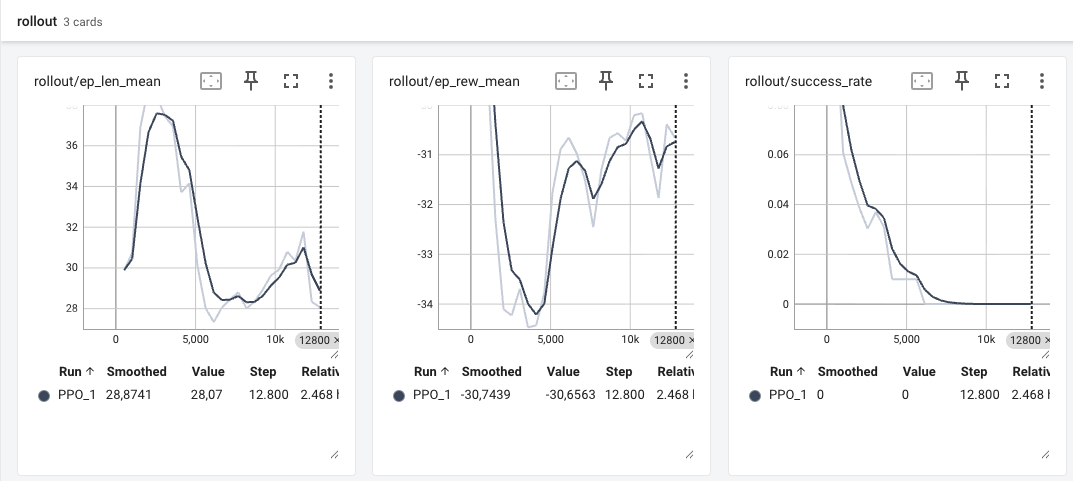
\includegraphics[width=0.95\textwidth]{images/tensorboard_exp010_rollout.png}
\caption{Métricas de \emph{rollout} de TensorBoard para Exp010. La tasa de éxito
desciende hasta cero y la recompensa media no muestra una tendencia sostenida de
mejora, por lo que la figura debe interpretarse como evidencia de diagnóstico y
no como demostración de aprendizaje estable.}
\label{fig:anexos:tensorboard_exp010_rollout}
\end{figure}

\begin{figure}[H]
\centering
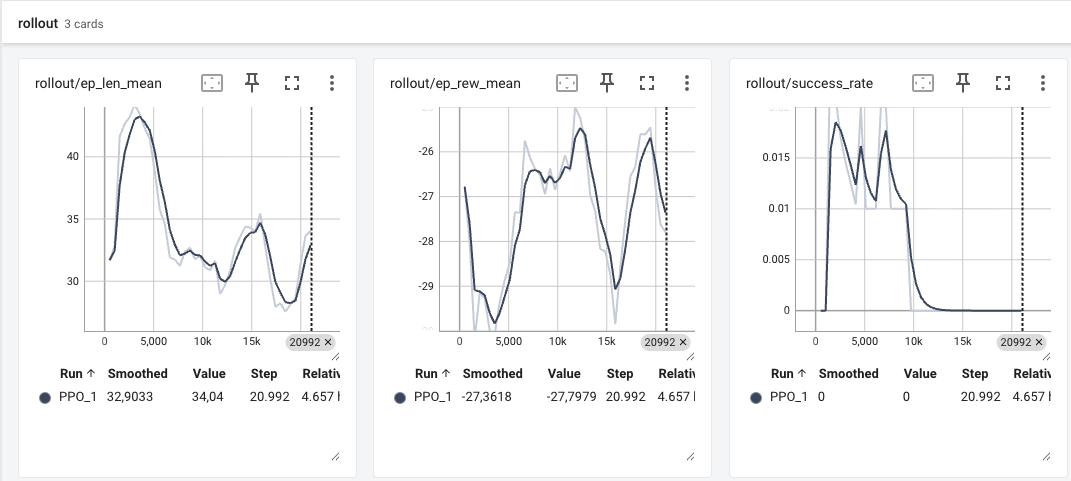
\includegraphics[width=0.95\textwidth]{images/tensorboard_exp011_rollout.png}
\caption{Métricas de \emph{rollout} de TensorBoard para Exp011. Aunque la
configuración reduce la saturación inicial y mejora parcialmente la recompensa
media frente a Exp010, la tasa de éxito vuelve a cero y las terminaciones por
límites o baja altitud siguen dominando el entrenamiento.}
\label{fig:anexos:tensorboard_exp011_rollout}
\end{figure}

\begin{figure}[H]
\centering
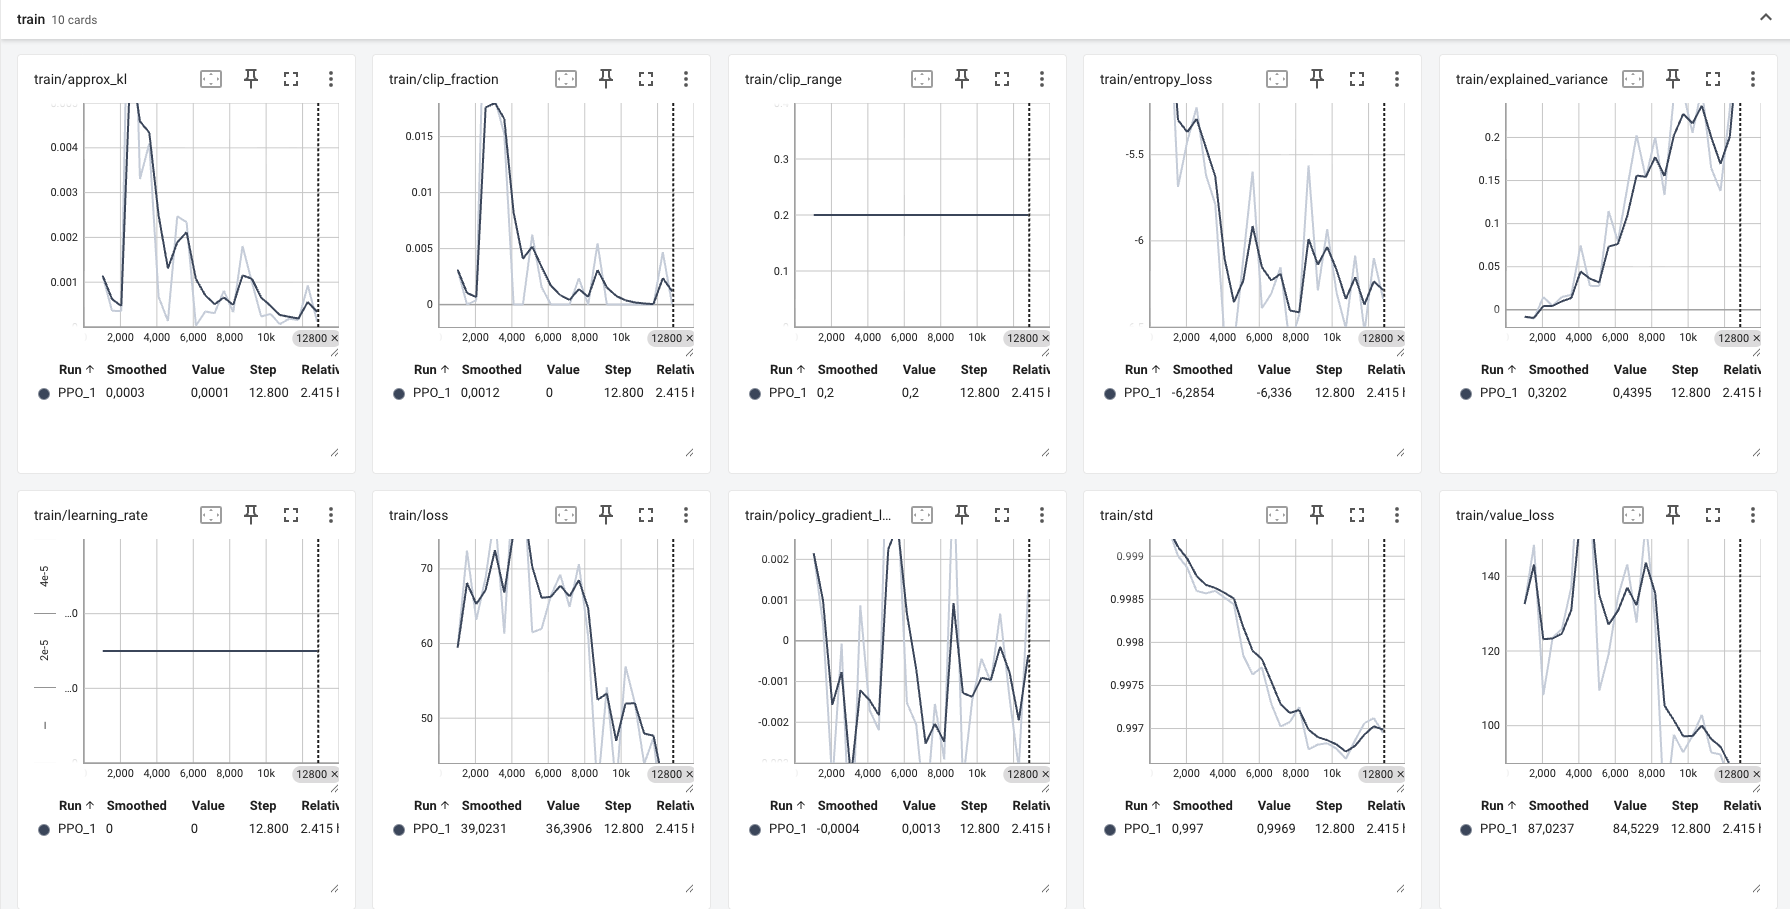
\includegraphics[width=0.95\textwidth]{images/tensorboard_exp010_train.png}
\caption{Métricas internas de PPO para Exp010. Los indicadores de entrenamiento
se mantienen en rangos razonables para una ejecución estable de PPO, pero esto no
implica éxito de la tarea cuando las métricas de episodio muestran predominio de
terminaciones no deseadas.}
\label{fig:anexos:tensorboard_exp010_train}
\end{figure}

\begin{figure}[H]
\centering
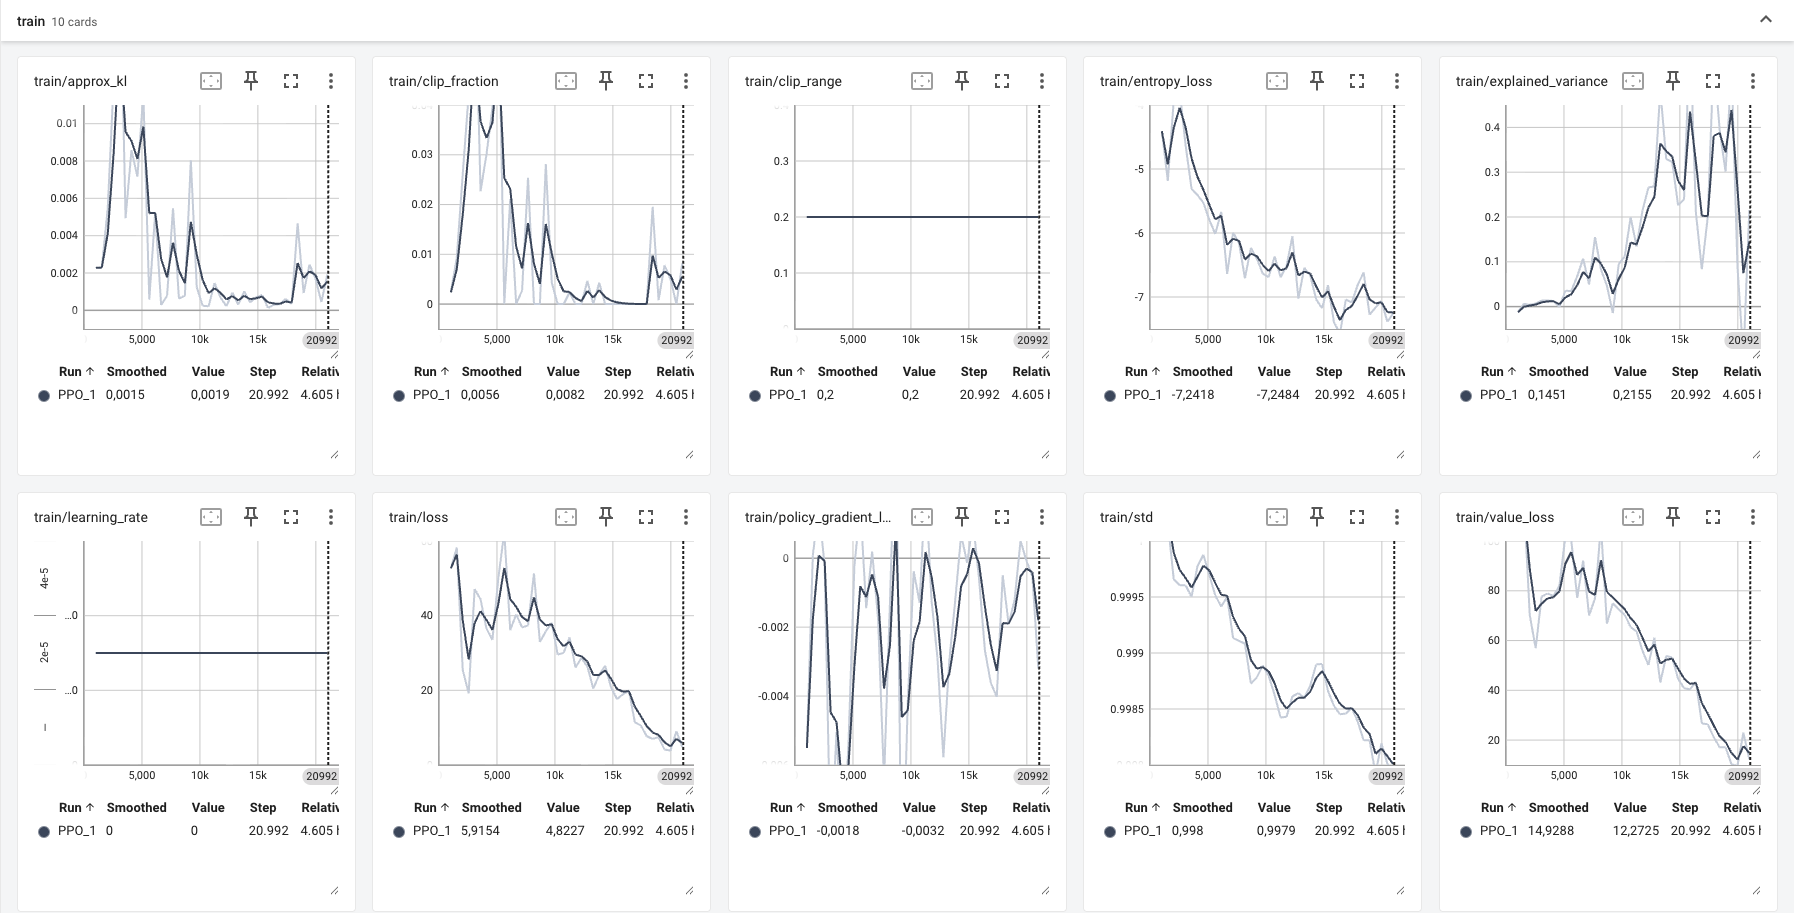
\includegraphics[width=0.95\textwidth]{images/tensorboard_exp011_train.png}
\caption{Métricas internas de PPO para Exp011. La evolución de pérdidas,
entropía y varianza explicada se utiliza como apoyo técnico, mientras que la
interpretación principal del experimento se obtiene de las métricas de
\emph{rollout} y de los monitores de episodio.}
\label{fig:anexos:tensorboard_exp011_train}
\end{figure}

\section{Declaración de uso de herramientas de inteligencia artificial} \label{sct:anexos:uso_ia}

Durante la realización del presente trabajo se han empleado herramientas de
inteligencia artificial generativa como apoyo a tareas de programación,
diagnóstico, organización de resultados y organización en la redacción. En particular, se ha
utilizado OpenAI Codex en el entorno de desarrollo para asistencia sobre código,
inspección del repositorio, generación de propuestas de modificación, revisión de
errores y apoyo a la edición de la memoria \cite{openai2026codex}. También se ha
utilizado ChatGPT como asistente conversacional para estructurar explicaciones,
revisar redacción y sintetizar criterios de presentación académica
\cite{openai2026chatgpt}.

El uso de estas herramientas no sustituye la autoría ni la responsabilidad
académica del trabajo. Las decisiones de diseño, la interpretación de resultados,
la selección de experimentos y la aceptación final de cambios se han revisado a
partir del repositorio, de las trazas de ejecución, de los ficheros de
configuración y de los logs experimentales. Las
respuestas generadas por IA se han tratado como propuestas de trabajo que debían
ser verificadas, corregidas o descartadas antes de incorporarse al documento o al
código.

\begin{table}[H]
\centering
\small
\setlength{\tabcolsep}{4pt}
\renewcommand{\arraystretch}{1.15}
\begin{tabular}{p{0.22\textwidth} p{0.32\textwidth} p{0.34\textwidth}}
\hline
\textbf{Herramienta} & \textbf{Tareas asistidas} & \textbf{Validación aplicada} \\
\hline
OpenAI Codex & Inspección del repositorio, edición de LaTeX, revisión de errores de compilación y apoyo a cambios de código. & Revisión manual de los diffs, compilación de LaTeX y contraste con el repositorio.\\
ChatGPT & Estructuración de explicaciones, síntesis de resultados y apoyo a redacción académica. & Revisión del texto, eliminación de afirmaciones no respaldadas y contraste con evidencias experimentales. \\
\hline
\end{tabular}
\caption{Resumen del uso de herramientas de inteligencia artificial generativa.}
\label{tab:anexos:uso_ia}
\end{table}

Entre los prompts más relevantes se encuentran los dirigidos a analizar 
el estado real del repositorio y del registro experimental, a
identificar diferencias entre resultados de entrenamiento y resultados de
infraestructura. Por otra parte para revisar la compilación LaTeX y para organizar la 
incorporación de figuras y tablas. 

No se han utilizado las herramientas de inteligencia artificial como fuente
bibliográfica primaria sobre aprendizaje por refuerzo, ROS 2, Aerostack2 o
Stable-Baselines3. Las afirmaciones técnicas del cuerpo de la memoria se apoyan
en referencias bibliográficas, documentación técnica, código implementado y
evidencia experimental. Cuando se ha incorporado texto redactado con apoyo de IA,
este se ha revisado y adaptado para mantener el tono académico, la precisión
terminológica y la coherencia con los resultados disponibles.

%%-----------------------------------------------
\end{document}
